%\section{Planification par compilation}
\section{Planification classique SAT et QBF}
%



%%%%%%%%%%%%%%%%%%%%%%%%%%%%%%%%%%%%%%%%%%%%%%%%%%%%%%%
%%%%%%%%%%%%%%%%%%%%%%%%%%%%%%%%%%%%%%%%%%%%%%%%%%%%%%%
%\subsection{Classical STRIPS Planning}
\subsection{Définitions préliminaires}
%%%%%%%%%%%%%%%%%%%%%%%%%%%%%%%%%%%%%%%%%%%%%%%%%%%%%%%
%%%%%%%%%%%%%%%%%%%%%%%%%%%%%%%%%%%%%%%%%%%%%%%%%%%%%%%

%In SAT planning, each copy of the variable set $X$ is indexed, making the writing of transitions easy; let $P$ and $Q$ two formulas and $x_i$ and $x_{i+1}$ two copies of one variable

\begin{definition}
Un \emph{problème de planification classique} STRIPS est un triplet $\langle \F, \I, \A , \G \rangle$ où $\F$ est un ensemble fini de \emph{fluents} (propositions atomiques), $\I \subseteq \F$ est l'ensemble initial de fluents, $\G \subseteq \F$ est l'ensemble des fluents buts et $\A$ est l'ensemble des actions.
Une action $\a \in \A$ est un triplet $\langle \Cond{\a}, \Add{\a}, \Del{\a} \rangle$ où

\begin{itemize}
\item $\Cond{\a} \subseteq \F$ est l'ensemble des fluents requis pour exécuter $\a$ (%les 
\emph{préconditions} de $\a$),
\item $\Add{\a} \subseteq \F$ et $\Del{\a} \subseteq \F$ sont les ensembles de fluents respectivement ajoutés et supprimés par l'action $\a$ (%les 
\emph{ajouts} et %les 
\emph{retraits} de $\a$).
\end{itemize}
\end{definition}

{\color{red}
%Les codages d'un problème de planification sous forme de base de clauses seront formalisés par des règles de réécriture. Ces règles seront exprimées par rapport à un problème de planification $\Pi=\langle F, A, I, B\rangle$ et un entier $k\geq 0$ qui représentera le nombre de niveaux des plans produits. Nous utiliserons également les sous-ensembles de $F$ suivants~: $F_p = \bigcup_{a\in   A} \mathrm{Prec}(A)$, $F_a = \bigcup_{a\in A} \mathrm{Add}(A)$, $F_d = \bigcup_{a\in A} \mathrm{Del}(A)$ dénotant respectivement les ensembles de fluents se trouvant en précondition, en ajout et en retrait des actions. Les règles des codages seront parfois exprimées sous forme non clausale pour des raisons de compacité, mais la transformation sous forme de clauses est immédiate.

Soient $A=\{a_1, \ldots, a_n\}$ un ensemble fini quelconque et $f$ une règle de
réécriture.  Pour une action $a\in A$, soit $P[a]$ une propriété que peut (ou
non) vérifier $a$. Soit $P_A=\{a\in A \suchthat P[a]\
\mathrm{vraie}\}=\{b_1,\ldots,b_m\}$~:
\begin{itemize}
\item $\biget{a\in A} f(a)$ dénote $F=f(a_1) \land\ldots\land f(a_n)$. Si $A=\emptyset$, alors $F=\top$.
\item $\bigou{a\in A} f(a)$ dénote $F=f(a_1) \lor\ldots\lor f(a_n)$. Si $A=\emptyset$, alors $F=\bot$.
\item $\biget{a\in A \suchthat P[a]} f(a)$ dénote $F=f(b_1) \land\ldots\land f(b_m)$. Si $P_A=\emptyset$, alors $F=\top$.
\item $\bigou{a\in A \suchthat P[a]} f(a)$ dénote $F=f(b_1) \lor\ldots\lor f(b_m)$. Si $P_A=\emptyset$, alors $F=\bot$.
\end{itemize}

Pour deux formules $F_1$ et $F_2$ et une propriété $P$, la règle de réécriture
« si $P$ est satisfaite, alors $F_1$ sinon $F_2$ » sera notée
$\ifthen{P}{F_1}{F_2}$.
}

\fred{Ensemble des variables d'actions $X_{\A}$}


\fred{A revoir:}
Nous allons montrer que pour l'approche QBF, au-delà des améliorations sur les solveurs, d'autres travaux doivent être menés pour mettre au point des codages plus performants. Comme nous l'avons indiqué plus haut, cela a été réalisé pour SAT avec des améliorations significatives. Nous présentons ici deux nouveaux codages d'arbres compacts CTE (Compact Tree Encoding) de problèmes de planification en QBF: CTE-EFA basé sur des frame-axiomes explicatifs dans un espace d'états, et CTE-OPEN basé sur des liens de causalité dans un espace de plans. \fred{dans le chapitre EXPERIMENTATIONS:} Nous les comparons au codage de l'état de l'art CTE-NOOP basé sur des actions No-op et proposé dans \cite{DBLP:conf/ecai/CashmoreFG12}. En termes de temps d'exécution par rapport aux problèmes de référence, CTE-EFA et CTE-OPEN sont toujours plus efficaces que CTE-NOOP.


%\begin{itemize}
%\item QBFEVAL’16: largest number of participants ever.
%\item QBF proof systems: theoretical frameworks of solving techniques.
%\item CDCL (clause learning) and expansion: orthogonal solving approaches.
%\item QBF solving by counterexample guided abstraction refinement (CEGAR) [CGJ+03, JM15b, JKMSC16, RT15].
%\item New approaches, e.g., Skolem function computation [RS16].
%\item 10 QBF-related papers at SAT 2016 conference (27\%).
%\end{itemize}

%The QBF approach seems to have several advantages: for comparable SAT / QBF encodings, the size of the generated formulas is more compact \cite{DBLP:conf/ecai/CashmoreFG12}, 

%QBF is a young field of research \cite{DBLP:conf/aaai/CadoliGS98} compared to SAT 
%\begin{itemize}
%\item progrès actuels des solveurs QBF (Qell 10 fois plus rapide sur planning-CTE (qu'est ce que ça veut dire ?) que rareqs, rareqs qui est 2 fois plus rapide que depqbf, chercher refs)
%\item ordre de performance des codages SAT (NOOP+GP, EFA, OPEN) et QBF (EFA, OPEN, NOOP) diffère
%\end{itemize}


%{\color{blue}
%At the time being the SAT approach is actually the best as SAT solvers and encodings have been greatly improved since 1992. So, it would be useless to compare QBF solvers to SAT solvers: the result of the contest is known in advance \cite{DBLP:phd/ethos/Cashmore13}. We believe that, nevertheless, QBF approach to automated planning deserves the interest of the community before it proves to be faster than SAT approach. Our paper shows that beyond the implementation of solvers, further work has to be done on the encodings.

%"Since the first complete QBF solver was presented decades after the first complete engine to solve SAT, research in this field remains at its infancy. compared to SAT (1960s), QBF still is a young field of research"
%}









%%%%%%%%%%%%%%%%%%%%%%%%%%%%%%%%%%%%%%%%%%%%%%%%%%%%%%%%%%%%%%%%%%%%%%%%%%%%%%%%
%%%%%%%%%%%%%%%%%%%%%%%%%%%%%
% PLANIFICATION SAT
%%%%%%%%%%%%%%%%%%%%%%%%%%%%%
\subsection{Codages SAT de référence pour la planification classique}
%

%
% codage SAT-EFA
%
%\subsection{Codage SAT de référence dans les espaces d'états}

\fred{Présenter le codage KS92,95 SAT-EFA classique}

\fred{Attention, ici copier/coller ouvrage SAT 2008 Maris, Régnier, Vidal}
{\color{red}

\subsubsection{Codage dans les espaces d'états avec frame-axiomes explicatifs}

\begin{figure}\label{steps:sat}
\begin{footnotesize}
%(a)\\[1em]

\fred{Rajouter la figure que j'ai enlevée ici !!!}
%   \xymatrix@C=0.1pc@R=1pc{
%   \text{S}_{0} (\textit{Init}) \ar@{->}[r] & \fbox{$x_{1}\equiv$ S$_{1}$} \ar@{>}[r]  & \fbox{$x_{2}\equiv$ S$_{2}$} \ar@{>}[r] & \fbox{$x_{3}\equiv$ S$_{3}$} \ar@{>}[r] & \fbox{$x_{4}\equiv$ S$_{4}$}
%   \ar@{>}[r] & \fbox{$x_{5}\equiv$ S$_{5}$} \ar@{>}[r] & \fbox{$x_{6}\equiv$ S$_{6}$} \ar@{>}[r] & \fbox{$x_{7}\equiv$ S$_{7}$} \ar@{>}[r] & \text{S}_{8} (\textit{Goal})
%   }
\end{footnotesize}
\vspace{1em}
\caption{Transitions of an 8-step plan in SAT/SMT encoding}
\end{figure}


Les codages dans les espaces d'états sont basés sur les transitions entre les étapes successives du plan en partant de l'état initial pour arriver au but.
%Le parallélisme y est codé grâce à la notion d'indépendance entre actions simultanées. 
Pour conserver les fluents non affectés par les actions qui doivent être exécutées dans une étape du plan, on va coder la notion de frame-axiome.
Nous décrivons d'abord la technique la plus efficace en termes de compacité et
de temps de résolution \cite{MK99} qui utilise des frame-axiomes explicatifs.
Nous présentons ensuite une variation de ce codage utilisant des actions
particulières appelées no-ops \cite{KMS96}.
Les règles du codage dans les espaces d'états produisent des propositions de la
forme $a(i)$ qui représentent le fait que l'action $a$ est appliquée à un niveau
$i$ du plan ssi $a(i)$ a la valeur de vérité vrai, et des propositions de la
forme $f(i)$ qui représentent le fait que le fluent $f$ est présent au niveau
$i$ ssi $f(i)$ a la valeur de vérité vrai. Le présence de $f$ au niveau $i$
signifie qu'il est présent après l'application successive de toutes les
actions associées à des propositions qui sont vraies, du niveau 1 jusqu'au
niveau $i$. Ce codage comporte cinq règles~:

} % FIN COLOR RED


%\begin{enumerate}
%\item \codrule
\paragraph*{[SAT-EFA.1 -- état initial et but]}
Les fluents de l'état initial sont vrais au niveau $0$ et ceux qui ne sont pas dans l'état initial sont faux au niveau $0$. Tous les fluents du but doivent être vrais au niveau $\length$.

  \codage{\noindent\left(\Bigforall{\f \in \I} \f_{0} \right) \land \left(\Bigforall{\f \in (\F \setminus \I)}\neg \f_{0} \right) \land \left(\Bigforall{\f \in \G}\f_{\length} \right)}
%\item \label{codage:ee2} \codrule
\paragraph*{[SAT-EFA.2 -- Préconditions et effets des actions]} %si une action appartient au plan, alors ses préconditions sont vérifiées et ses effets sont produits.
Si une action $\a$ est exécutée dans une transition du plan (au niveau $i$), alors chaque effet de $\a$ se produit dans l'état résultant (au niveau $i$) et chaque précondition de $\a$ est requise dans l'état précédent (au niveau $i-1$).
  \codage{\BigforallTwo{i=1}{\length} \Bigforall{\a \in \A} \left(
      \a_{i} \Rightarrow \left( \Bigforall{\f \in \Cond{\a}} \f_{i-1} \right) \land
      \left( \Bigforall{\f \in \Add{\a}} \f_{i} \right) \land \left( \Bigforall{\f
          \in \Del{\a}} \neg \f_{i} \right) \right)}
%\item \label{codage:ee4} \codrule
\paragraph*{[SAT-EFA.3 -- Frame-axiomes explicatifs]} %d'ajout]} %si un fluent devient vrai entre deux niveaux successifs du plan, alors une action au moins qui l'établit doit avoir été appliquée.  Il faut que le fluent puisse ne pas exister à un instant donné, donc ne pas appartenir à $I$ ou appartenir à $F_d$. Il lui faut aussi pouvoir être ajouté par une action donc appartenir à $F_a$.
Si la valeur d'un fluent change entre deux états consécutifs (du niveau $i-1$ au niveau $i$), alors une action qui produit cette modification est exécutée dans la transition du plan entre ces états (au niveau $i$).
  \codage{\BigforallTwo{i=1}{\length} \Bigforall{\f \in \F} \left( \neg \f_{i-1} \land \f_{i} \Rightarrow \Bigexists{\substack{\a \in \A \\ \f \in \Add{\a}}} \a_{i} \right)}
%\item \label{codage:ee3} \codrule
%\paragraph*{[SAT-EFA.3.2 -- Frame-axiomes explicatifs de retrait]} si un fluent devient faux entre deux niveaux successifs du plan, alors une action au moins qui le retire doit avoir été appliquée. Il faut que le fluent existe à un instant donné, il doit donc appartenir à $I$ ou à $F_a$. Il lui faut aussi pouvoir être retiré par une action, il doit donc aussi appartenir à $F_d$.
 \codage{\BigforallTwo{i=1}{\length} \Bigforall{\f \in \F} \left( \f_{i-1} \land \neg \f_{i} \Rightarrow \Bigexists{\substack{\a \in \A \\ \f \in \Del{\a}}} \a_{i} \right)}
%\item \label{codage:ee5} \codrule
\paragraph*{[SAT-EFA.4 -- Prévention des interactions négatives]}%Interférences]} %deux actions non indépendantes ne peuvent pas être exécutées au même niveau. 
Les effets contradictoires sont déjà pris en compte par la règle SAT-EFA.2.
Cette règle doit donc seulement empêcher les interactions entre les préconditions et les retraits des actions. Si une action supprime un fluent nécessaire à une autre action, ces deux actions ne peuvent pas être exécutées dans une même transition du plan.

%\begin{scriptsize}
\[ \BigforallTwo{i=0}{\depth} \Bigforall{\a \in \A} \Bigforall{\f\in \Cond{\a}} \Bigforall{\b \in \A \\ \a \neq \b \\ \f \in \Del{\b}}\left(\neg \a_{i} \vee \neg \b_{i}\right) \]
%\end{scriptsize}  
%  \codage{\biget{i \in [1,k]} \biget{\{a_m, a_n\} \subseteq A \suchthat m < n \land (a_m\|_e a_n) \land \lnot (a_m\|_i a_n)} \left[ \neg a_m(i) \lor \neg a_n(i) \right]}
%\end{enumerate}



%
% codage SAT-MK99-ESPACES-DE-PLAN
%
\subsection{Codages SAT de référence dans les espaces de plans}

\fred{Présenter les codages MK99 espaces de plans}

\fred{Attention, ici copier/coller ouvrage SAT 2008 Maris, Régnier, Vidal}
{\color{red}
Ces codages ne traduisent plus seulement les transitions qui s'opèrent entre niveaux successifs du plan, mais expriment maintenant les relations de causalité entre les actions qui le constituent. Dans les espaces d'états, l'application des actions est envisagée séquentiellement~: une action ne peut apparaître à un niveau du plan que lorsque ses préconditions sont satisfaites au niveau précédent.  Dans les espaces de plans, une action apparaît à un niveau du plan parce qu'une action d'un niveau antérieur (pas forcément le niveau précédent) établit ses préconditions et qu'une action qui suit requiert un de ses effets.
L'existence de différents codages découle de la traduction des différentes
stratégies de recherche utilisées dans les espaces de plans. Ces codages restent moins performants, en termes de compacité et de temps de résolution, que le meilleur codage dans les espaces d'états (celui avec frame-axiomes explicatifs)
\cite{MK99}.

Dans tous ces codages, les ensembles d'actions indépendants qui peuvent faire partie d'un plan sont associés à des symboles d'étapes. Un ordre sur ces étapes détermine un ordre total pour l'exécution des ensembles d'actions indépendants.
Deux étapes particulières sont créées~: l'étape $\step{0}$ qui représente l'état initial du problème, et l'étape $\step{k+1}$ qui représente le but du problème. Ces deux étapes ne contiendront aucune action. Elles sont équivalentes aux actions fictives $Start$ et $End$ qui servent à initialiser un plan partiel et sont généralement utilisées en planification dans les espaces de plans partiels. Pour prendre en
compte ces deux étapes, l'ensemble $F_a$ des fluents présents dans les ajouts des actions est augmenté des fluents de l'état initial $I$. De même, l'ensemble $F_p$ des fluents présents dans les préconditions des actions est augmenté des fluents du but $B$. On peut produire des codages produisant moins de clauses en considérant les actions $Start$ et $End$ comme des cas particuliers \cite{Vid01}, mais pour des raisons de compacité dans l'écriture des codages nous les présentons ici de manière intégrée aux autres actions.

Les règles des codages dans les espaces de plans produisent les propositions suivantes, pour une action $\a$, un fluent $\f$, et deux étapes $\step{i}$ et $\step{j}$~:

\begin{itemize}
\item $(\a \in \step{i})$ est vraie ssi l'action $\a$ appartient à l'étape $\step{i}$.
\item $\Adds{i}{\f}$, est vraie ssi l'étape $\step{i}$ contient une action qui ajoute le
  fluent $\f$.
\item $\Needs{i}{\f}$ est vraie ssi l'étape $\step{i}$ contient une action qui a $f$ en
  précondition.
\item $\Dels{i}{\f}$ est vraie ssi l'étape $\step{i}$ contient une action qui retire le
  fluent $\f$.
\item $\Linksteps{i}{\f}{j}$ représente un lien causal et est vraie ssi l'étape
  $\step{i}$ produit le fluent $\f$ qui est une précondition de l'étape $\step{j}$.
\item $\step{i} \prec \step{j}$ est vraie ssi l'étape $\step{i}$ précède l'étape $\step{j}$~; toutes les actions
  associées à $\step{i}$ doivent donc être exécutées avant celles associées à $\step{j}$.
  Ces propositions traduisent un ordre partiel sur les étapes.
\end{itemize}


\subsubsection{Partie commune des codages dans les espaces de plans}

Elle permet d'établir une correspondance entre toutes les actions disponibles et
celles qui font partie des étapes des plans solutions. Elle est constituée
de cinq règles~:


%\begin{enumerate}
%\item 
%\tagrule{SAT/PS-MK99.1}\codrule
\paragraph*{[SAT-CL.1 -- état initial et but]} l'étape $\step{0}$ produit l'état
  initial du problème, et l'étape $\step{k+1}$ requiert les buts.
  \codage{\left( \Bigforall{\f \in \I}\Adds{0}{\f}\right) \land \left( \Bigforall{\f \in (\F\setminus \I)}\lnot\Adds{0}{\f}\right) \land \left( \Bigforall{\f \in \G} \Needs{k+1}{\f}\right)\label{codage:epcom1}}
%\item 
%\tagrule{SAT/PS-MK99.2}\codrule
\paragraph*{[SAT-CL.2 -- Correspondance action/étape]} si une étape ajoute, retire, ou a
  pour précondition un fluent, alors cette étape peut correspondre à n'importe
  quelle action qui a le même comportement vis-à-vis de ce fluent. Inversement,
  si une action appartient à une étape, ses préconditions, ajouts et retraits
  sont vrais.

  \codage{\BigforallTwo{i=1}{k} \Bigforall{\f \in \F} \begin{pmatrix}
  \left( \Adds{i}{\f} \Leftrightarrow \Bigexists{\substack{\a \in \A \\\f \in \Add{\a}}} \instep{\a}{i} \right)
  \wedge \left( \Dels{i}{\f} \Leftrightarrow \Bigexists{\substack{\a \in \A \\\f \in \Del{\a}}} \instep{\a}{i} \right)\\
  \wedge \left( \Needs{i}{\f} \Leftrightarrow \Bigexists{\substack{\a \in \A \\\f \in \Cond{\a}}} \instep{\a}{i} \right)
  \end{pmatrix}}

%  \codage{\BigforallTwo{i=1}{k} \Bigforall{\f \in \F} \left( \Adds{i}{\f} \Leftrightarrow \Bigexists{\substack{\a \in \A \\\f \in \Add{\a}}} \instep{\a}{i} \right)\label{codage:epcom2}}
%  \codage{\BigforallTwo{i=1}{k} \Bigforall{\f \in \F} \left( \Dels{i}{\f} \Leftrightarrow \Bigexists{\substack{\a \in \A \\\f \in \Del{\a}}} \instep{\a}{i} \right)\label{codage:epcom3}}
%  \codage{\BigforallTwo{i=1}{k} \Bigforall{\f \in \F} \left( \Needs{i}{\f} \Leftrightarrow \Bigexists{\substack{\a \in \A \\\f \in \Cond{\a}}} \instep{\a}{i} \right)\label{codage:epcom4}}
%\item 
%\tagrule{SAT/PS-MK99.3}\codrule
%\paragraph*{[SAT-MK99.3 -- Exclusions mutuelles]} deux actions qui ne sont pas indépendantes ne peuvent appartenir à une même étape.
%  \codage{\biget{i \in [1,k]} \biget{ \{a_m, a_n\} \subseteq A \suchthat m < n \land \lnot(a_m\|a_n)} \left[\neg (a_m \in p_i) \lor \neg(a_n \in p_i) \right]\label{codage:epcom5}}
%\end{enumerate}

\paragraph*{[SAT-CL.3 -- Prévention des interactions négatives]}
Si une action supprime un fluent qui est nécessaire ou est ajouté par une autre action, alors ces deux actions ne peuvent pas être exécutées toutes les deux dans une même étape.

\begin{small}
\[
\BigforallTwo{i=1}{k}\Bigforall{\substack{\a\in \A}}\Bigforall{\substack{\f\in \left(\Add{\a}\cup\Cond{\a}\right)}}\Bigforall{\substack{\b\in \A\\\a \neq \b \wedge \f \in \Del{\b}}}\left(\neg \instep{\a}{i} \vee \neg \instep{\b}{i}\right)
\]
\end{small}

\subsubsection{Codage par liens causaux, protection d'intervalles et ordre partiel}

La production des préconditions se fait par le codage direct des liens causaux.
La proposition $\Linksteps{i}{\f}{j}$ traduit le fait que l'étape $\step{i}$ produit le fluent
$\f$, précondition de l'étape $\step{j}$. La protection de $\f$ dans l'intervalle compris
entre les deux étapes se fait par promotion (l'étape menaçant $\f$ est placée
avant $\step{i}$), ou par rétrogradation (l'étape menaçant $\f$ est placée après $\step{j}$).
L'ordre d'exécution des étapes  est donné par une relation de précédence de
la forme $\step{i} \prec \step{j}$. Les quatre règles suivantes sont ajoutées à la partie commune~:

%\begin{enumerate}
%\item \codrule
\paragraph*{[SAT-CLPO.4 -- Production des préconditions]} chaque fluent est supporté par un lien
  causal entre l'étape qui le produit et l'étape
  qui l'utilise en tant que précondition.
  \codage{\BigforallTwo{i=1}{k+1} \Bigforall{\f\in \F} \left( \Needs{i}{\f} \Rightarrow %\ifthen{\f \in \F_a}{
  \BigexistsTwo{\substack{j=0\\j\neq i}}{k} \Linksteps{j}{\f}{i}%}{\bot}
  \right)}
%\item \codrule
\paragraph*{[SAT-CLPO.5 -- Liens causaux]} un lien causal supportant un fluent $\f$ entre
  deux étapes $\step{i}$ et $\step{j}$ implique que $\step{i}$ ajoute $\f$, que $\step{j}$ a pour
  précondition $\f$, et que $\step{i}$ précède $\step{j}$.
  \codage{\BigforallTwo{i=0}{k} \BigforallTwo{\substack{j=1\\j\neq i}}{k+1} \Bigforall{\f\in \F} \left( \Linksteps{i}{\f}{j} \Rightarrow\left( \Adds{i}{\f} \land \Adds{j}{\f}\land \step{i} \prec \step{j}  \right) \right)}
%\item \codrule
\paragraph*{[SAT-CLPO.6 -- Protection d'intervalles]} si un lien causal supporte le
  fluent $\f$ entre une étape $\step{i}$ et une étape $\step{j}$, et si une étape $\step{q}$
  retire $\f$, alors $\step{q}$ doit précéder $\step{i}$ (promotion) ou $\step{j}$ doit précéder
  $\step{q}$ (rétrogradation).
  \codage{\BigforallTwo{i=0}{k} \BigforallTwo{\substack{j=1\\j\neq i}}{k+1} \BigforallTwo{\substack{q=1\\q\neq i \land q\neq j}}{k} \Bigforall{\f\in \F} 
  \left( %\begin{array}{l}
  \Linksteps{i}{\f}{j} \land \Dels{q}{\f} \Rightarrow%\\
  \left( \step{q} \prec \step{i} \lor \step{j} \prec \step{q} \right) %\end{array}
  \right)}
%\item \codrule
\paragraph*{[SAT-CLPO.7 -- Propriétés de la relation de précédence]} transitive et
  antisymétrique. L'irréflexivité est codée dans les autres règles par le biais
  des indices des étapes.
  \codage{\BigforallTwo{i=0}{k+1} \BigforallTwo{\substack{j=0\\j\neq i}}{k+1} \BigforallTwo{\substack{q=0\\q\neq i \land q\neq j}}{k+1} \left( \left( \step{i} \prec \step{j} \land \step{j} \prec \step{q} \right) \Rightarrow \step{i} \prec \step{q} \right)}
  \codage{\BigforallTwo{i=0}{k} \BigforallTwo{\substack{j=i+1\\j\neq i}}{ k+1} \lnot \left( \step{i} \prec \step{j} \right) \lor \lnot \left( \step{j} \prec \step{i} \right)}
%\end{enumerate}

\subsubsection{Codage par liens causaux, protection d'intervalles et étapes contiguës}

Ce codage simplifie le précédent dans lequel plusieurs modèles correspondent au
même plan solution, à la numérotation des étapes près. Les étapes doivent
maintenant suivre un ordre prédéfini d'indice croissant, ce qui rend inutile la
relation de précédence. La protection d'intervalles ne nécessite plus la
promotion ou la rétrogradation avec un ordre partiel sur les étapes, mais se
réalise en interdisant qu'une étape comprise dans un intervalle défini par un
lien causal ne le menace. Les deux règles suivantes sont ajoutées à la partie
commune~:

%\begin{enumerate}
%\item \codrule
\paragraph*{[SAT-CLCS.4 -- Production des préconditions]} chaque fluent est supporté par un
  lien causal entre l'étape qui le produit et l'étape qui l'utilise en tant que
  précondition.
  \codage{\BigforallTwo{i=1}{k} \Bigforall{\f\in \F} \left( \Needs{i}{\f} \Rightarrow %\ifthen{\f \in \F_a}{
  \BigexistsTwo{j=1}{i-1} \Linksteps{j}{\f}{i}%}{\bot}
  \right)}
%\item \codrule
\paragraph*{[SAT-CLCS.5 -- Liens causaux et protection d'intervalles]} la présence d'un lien
  causal supportant un fluent $\f$ entre deux étapes $\step{i}$ et $\step{j}$
  implique que $\step{i}$ ajoute $\f$ et que $\step{j}$ a pour précondition
  $\f$. De plus, une étape qui retire $\f$ ne peut s'insérer entre $\step{i}$ et $\step{j}$.
%  \codage{
\[
\BigforallTwo{i=1}{k-1} \BigforallTwo{j=i+1}{k} \Bigforall{\f\in \F} \left( %\begin{array}{l} 
  \Linksteps{i}{\f}{j} \Rightarrow \Adds{i}{\f} \land \Needs{j}{\f} \land %\\ %\ifthen{f \in F_d}{
  \BigforallTwo{q=i+1}{j-1} \lnot \Dels{q}{\f}%}{\top}
  %\end{array}
  \right)
\]
  %}
%\end{enumerate}

\subsubsection{Codage du \enquote{chevalier blanc}}

Ce codage est actuellement le plus compact des codages dans les espaces de plans
en nombre de variables et de clauses produites~; il est également le plus
performant par son temps de résolution. Il exprime directement les liens
causaux~: si une étape requiert un fluent, c'est qu'une étape précédente doit
l'avoir créé. On n'utilise ainsi que les variables déjà présentes dans la partie
commune. La protection d'intervalles se réalise en codant la technique du
\enquote{chevalier blanc} introduite par le planificateur \textsc{Tweak}
\cite{Cha87}. Les deux règles suivantes sont ajoutées à la partie commune~:


%\begin{enumerate}
%\item \codrule
%\tagrule{SAT/WK.1}\codrule
\paragraph*{[SAT-CLWK.4 -- Production des préconditions]} La précondition d'une étape d'un niveau
  $i$ doit être ajoutée par une étape précédente.
  \codage{\BigforallTwo{i=1}{k+1} \Bigforall{\f\in \F} \left( \Needs{i}{\f} \Rightarrow %\ifthen{f \in F_a}{
  \BigexistsTwo{j=0}{i-1} \Adds{j}{\f}%}{\bot}
  \right)}

%\item \codrule
%\tagrule{SAT/WK.2}\codrule
\paragraph*{[SAT-CLWK.5 -- Chevalier blanc]} Si une étape a pour précondition le fluent $f$
  au niveau $i$, et qu'une autre le retire au niveau $j$ avant que la première
  puisse l'utiliser, alors il doit y avoir une troisième étape qui rétablit $f$
  à un niveau $q$ tel que $j < q < i$.
  \codage{\BigforallTwo{i=3}{k+1} \BigforallTwo{j=1}{i-2} \Bigforall{\f \in \F} \left( %\begin{array}{l}
  \Needs{i}{\f} \land \Dels{j}{\f} \Rightarrow%\\ 
        %\ifthen{f \in F_a}{
        \BigexistsTwo{q=j+1}{i-1} \Adds{q}{\f}%}{\bot}
        %\end{array}
        \right)}
%\end{enumerate}

} % FIN COLOR RED


%
% codage SAT-OPEN
%
\subsection{Nouveau codage SAT dans les espaces de plans}

\fred{A ajouter: complexité en espace meilleure par rapport à MK99}

Les codages SAT dans les espaces de plans existants introduits par \cite{DBLP:conf/aaai/MaliK99} se r\'{e}f\`{e}rent tous \`{a} trois \'{e}tapes index\'{e}es (pas n\'{e}cessairement cons\'{e}cutives) du plan.
Dans notre nouveau codage, nous allons nous r\'{e}f\'{e}rer seulement \`{a} deux \'{e}tapes cons\'{e}cutives.
Pour chaque action $\a\in\A$ et chaque \'{e}tape $i$, nous cr\'{e}ons une variable propositionnelle $\a_{i}$ pour d\'{e}terminer qu'une instance de $\a$ doit \^{e}tre planifi\'{e}e \`{a} l'\'{e}tape $i$.
Pour chaque fluent $\f\in\F$ et chaque \'{e}tape $i$, nous cr\'{e}ons une variable propositionnelle $\open{\f}{i}$ pour exprimer que $\f$ se maintient \`{a} l'\'{e}tape pr\'{e}c\'{e}dente $i-1$ et doit \^{e}tre prot\'{e}g\'{e} au moins jusqu'\`{a} l'\'{e}tape $i$.

\begin{figure}[hb!]\centering
	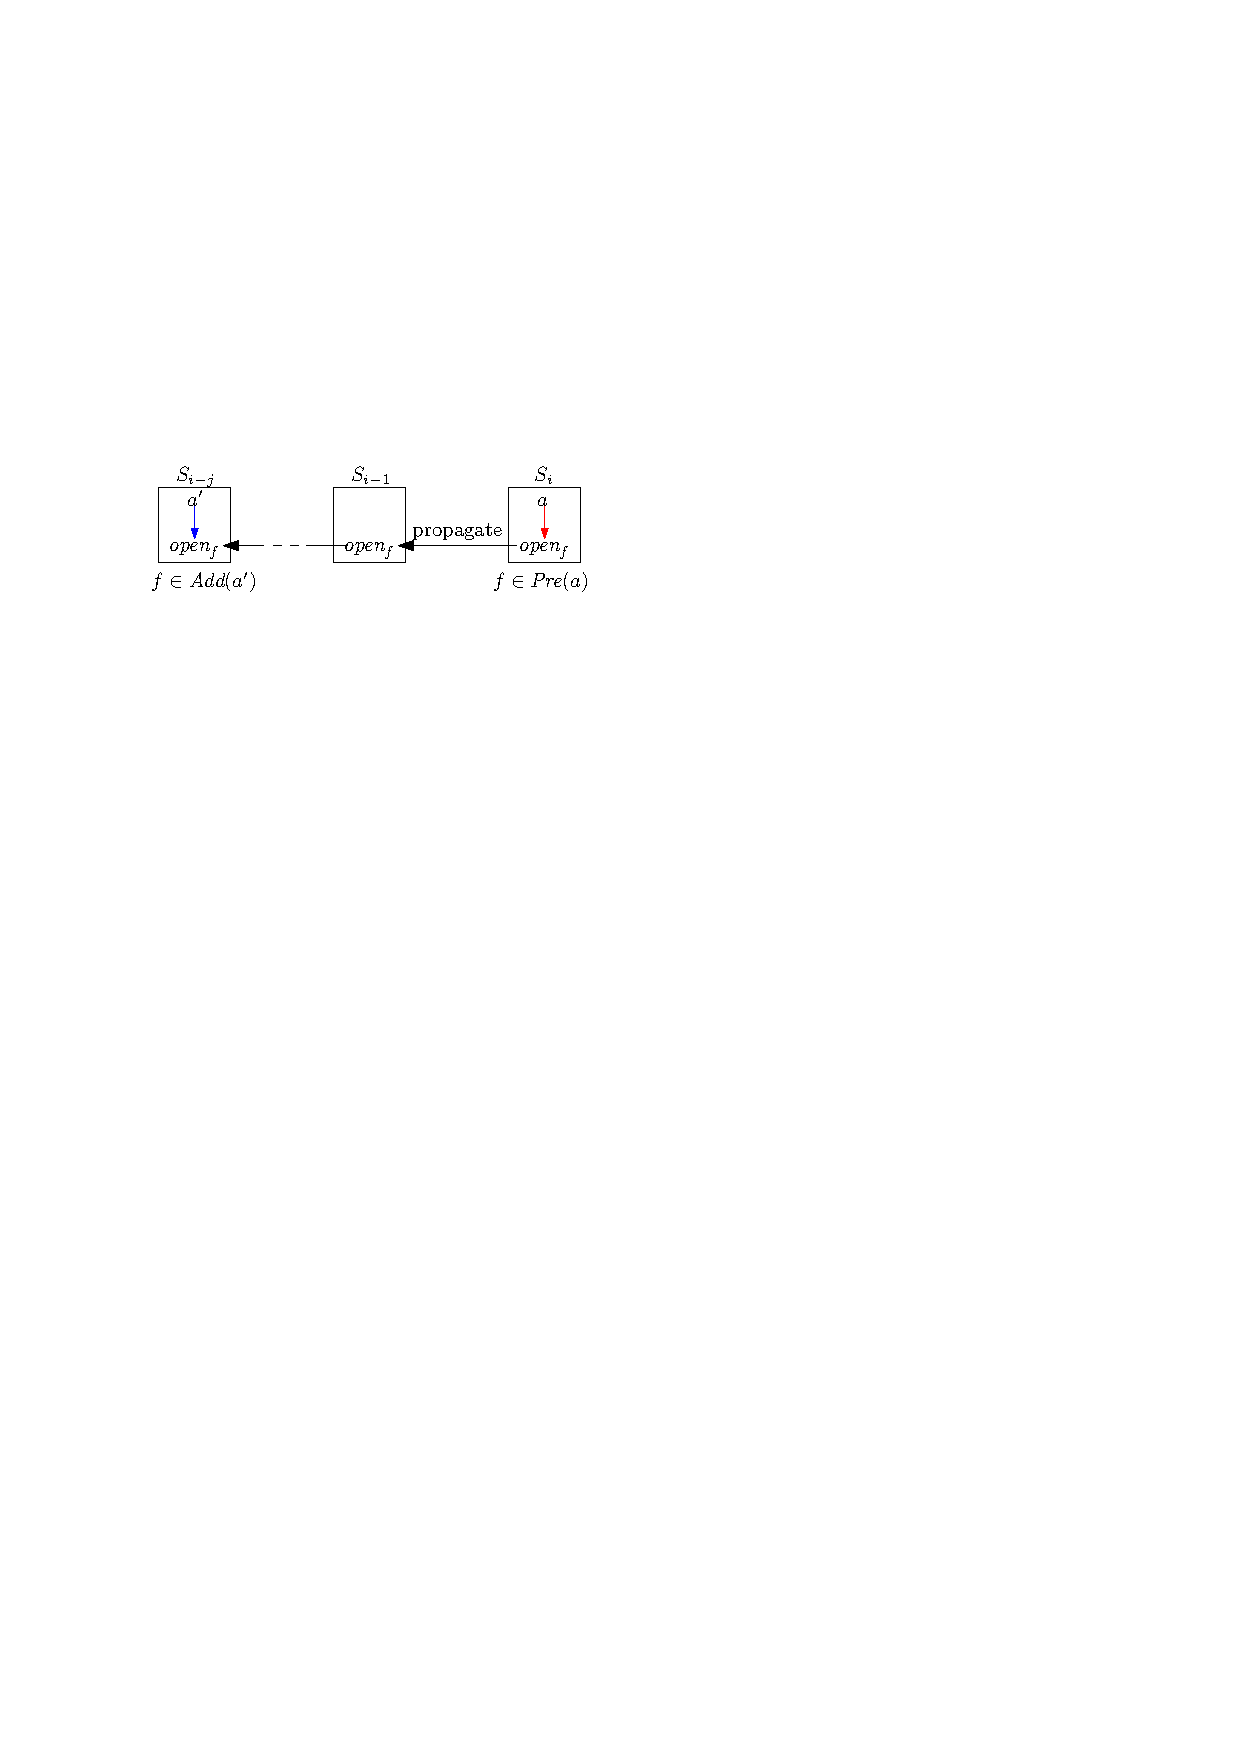
\includegraphics[width=.4\textwidth]{figures/transitions}
    \caption{Lien causal: l'action $a'$ produit $\f$ \`{a} l'\'{e}tape $S_{i-k}$ pour l'action $\a$ qui n\'{e}cessite $\f$ \`{a} l'\'{e}tape $S_{i}$.}
    \label{fig:causal-link}
\end{figure}

Dans la figure~\ref{fig:causal-link}, la variable $f$ est une \textit {condition ouverte} \`{a} l'\'{e}tape $\S_i$, impliquant que $\f\in\I$ ou une action $a'$ qui ajoute $\f$ est ex\'{e}cut\'{e}e dans une \'{e}tape pr\'{e}c\'{e}dente $\S_{i-k}$.
Les conditions ouvertes doivent \^{e}tre propag\'{e}es vers l'arri\`{e}re jusqu'\`{a} l'\'{e}tat initial ou une \'{e}tape dans laquelle elles sont ajout\'{e}es par une action.




%\paragraph*{SAT Encodings for Classical Planning}
%%\begin{figure}\label{steps:sat}
%%\begin{tiny}
%%%(a)\\[1em]
%%  \xymatrix@C=0.1pc@R=1pc{
%%  \text{S}_{0} (\textit{Init}) \ar@{>}[r] & \fbox{$x_{1}\equiv$ S$_{1}$} \ar@{>}[r]  & \fbox{$x_{2}\equiv$ S$_{2}$} \ar@{>}[r] & \fbox{$x_{3}\equiv$ S$_{3}$} \ar@{>}[r] & \fbox{$x_{4}\equiv$ S$_{4}$}
%%  \ar@{>}[r] & \fbox{$x_{5}\equiv$ S$_{5}$} \ar@{>}[r] & \fbox{$x_{6}\equiv$ S$_{6}$} \ar@{>}[r] & \fbox{$x_{7}\equiv$ S$_{7}$} \ar@{>}[r] & \text{S}_{8} (\textit{Goal}) \\
%%  }
%%\end{tiny}
%%%(b)\\[1em]
%%%   \hspace{0.8em}\xymatrix@C=0pc@R=1pc{
%%%   & & & & & \fbox{$x_{2}\equiv$ S$_{4}$} \ar@{.}[lld] \ar@{.}[rrd] \ar@/^1pc/[rdd] & & & & \\
%%%   & & & \fbox{$x_{1}\equiv$ S$_{2}$} \ar[rd] & & & & \fbox{$x_{1}\equiv$ S$_{6}$} \ar[rd] & & \\
%%%   \text{S}_{0} (\textit{Init}) \ar@{>}[rr] & & \fbox{$x_{0}\equiv$ S$_{1}$} \ar[ru]  & & \fbox{$x_{0}\equiv$ S$_{3}$} \ar@/^1pc/[ruu] & &  \fbox{$x_{0}\equiv$ S$_{5}$} \ar[ru] & & \fbox{$x_{0}\equiv$ S$_{7}$} \ar@{>}[rr] & & \text{S}_{8} (\textit{Goal}) \\
%%%  }
%%\vspace{1em}
%%\caption{Transitions of an 8-steps plan in SAT/SMT encoding}
%%\end{figure}
%  Each step $i$ is associated with:\hfill
%  \begin{itemize}
%    \item a set of propositional variables for actions $\{a_{i}^{1},a_{i}^{2}\ldots,a_{i}^{m}\}$
%    \item a set of propositional variables for open conditions $\{open_{f^1,i},open_{f^2,i},\ldots,open_{f^n,i}\}$ %which determine their value in state $x_{i-1}$
%  \end{itemize}


%\begin{frame}{SAT Encoding: open conditions}
%Given a propositional formula $\varphi$, $\textit{open}_{\varphi} = \textit{NNF}_{\textit{open}}(+1,\varphi)$ with:\\[0.8em]
%\begin{itemize}
%  \item $\textit{NNF}_{\textit{open}}(+1,f) = \textit{open}_{f}$
%  \item $\textit{NNF}_{\textit{open}}(-1,f) = \textit{open}_{\neg f}$\\[0.8em]
%  \item $\textit{NNF}_{\textit{open}}(+1,\neg \varphi) = \textit{NNF}_{\textit{open}}(-1,\varphi)$
%  \item $\textit{NNF}_{\textit{open}}(-1,\neg \varphi) = \textit{NNF}_{\textit{open}}(+1,\varphi)$\\[0.8em]
%  \item $\textit{NNF}_{\textit{open}}(+1,\varphi_{1} \wedge \varphi_{2}) = \textit{NNF}_{\textit{open}}(+1,\varphi_{1}) \wedge \textit{NNF}_{\textit{open}}(+1,\varphi_{2})$
%  \item $\textit{NNF}_{\textit{open}}(-1,\varphi_{1} \wedge \varphi_{2}) = \textit{NNF}_{\textit{open}}(-1,\varphi_{1}) \vee \textit{NNF}_{\textit{open}}(-1,\varphi_{2})$\\[0.8em]
%   \item $\textit{NNF}_{\textit{open}}(+1,\varphi_{1} \vee \varphi_{2}) = \textit{NNF}_{\textit{open}}(+1,\varphi_{1}) \vee \textit{NNF}_{\textit{open}}(+1,\varphi_{2})$
%   \item $\textit{NNF}_{\textit{open}}(-1,\varphi_{1} \vee \varphi_{2}) = \textit{NNF}_{\textit{open}}(-1,\varphi_{1}) \wedge \textit{NNF}_{\textit{open}}(-1,\varphi_{2})$\\[0.8em]
%\end{itemize}
%\end{frame}


%\paragraph*{SAT Encoding: open conditions, then propagate or close}

Dans la suite, nous donnons notre codage pour une longueur de plan fix\'{e}e $\length$. Une borne sup\'{e}rieure pour $\length$ est le nombre total d'\'{e}tats possibles, soit $2^{\mid\F\mid}$.

\paragraph*{Conditions ouvertes}

Si une action $\a$ est ex\'{e}cut\'{e}e dans une \'{e}tape du plan, alors chaque condition de $\a$ doit \^{e}tre une condition ouverte \`{a} cette \'{e}tape (c'est-\`{a}-dire qu'un lien causal est requis pour cette condition).


\begin{small}
\begin{multline*}
~\\[-3em]
\bigwedge\limits_{\substack{\mathbf{i}\in [1..\mathbf{\length}]}}\bigwedge\limits_{\substack{\mathbf{\a}\in \mathbf{\A}}}\left(\mathbf{\a}_{\mathbf{i}} \Rightarrow \bigwedge\limits_{\substack{\mathbf{\f}\in \pre{\mathbf{\a}}}}open_{\mathbf{\f},\mathbf{i}}\right)\hfill\\[-2em]
%%%
\end{multline*}
\end{small}

Dans la derni\`{e}re \'{e}tape du plan menant au but tous les fluents du but doivent \^{e}tre des conditions ouvertes ou ajout\'{e}es par des actions ex\'{e}cut\'{e}es dans cette \'{e}tape.

\begin{small}
\begin{multline*}
~\\[-3em]
\bigwedge\limits_{\substack{\mathbf{\f}\in \mathbf{\G}}}\left(open_{\mathbf{\f},\mathbf{\length}} \vee \bigvee\limits_{\substack{\mathbf{\a}\in \mathbf{\A}\\\mathbf{\f} \in \add{\mathbf{\a}}}}\mathbf{\a}_{\mathbf{\length}}\right)\hfill\\[-2em]
%%%
\end{multline*}
\end{small}

\paragraph*{Propagation et fermeture}

Aucune condition ne doit rester ouverte dans la premi\`{e}re \'{e}tape du plan si elle n'est pas fournie dans l'\'{e}tat initial.
%$\bigwedge_{\mathbf{\f}\in \mathbf{\F}\setminus \mathbf{I}}\neg open_{\mathbf{\f},1}$

\begin{small}
\begin{multline*}
~\\[-3em]
\bigwedge\limits_{\substack{\mathbf{\f}\in \mathbf{\F}\setminus \mathbf{I}}}\neg open_{\mathbf{\f},1}\hfill\\[-2em]
%%%
\end{multline*}
\end{small}

Toute condition ouverte dans une \'{e}tape doit soit rester ouverte soit \^{e}tre ajout\'{e}e (ferm\'{e}e) par une action \`{a} l'\'{e}tape pr\'{e}c\'{e}dente.

\begin{small}
\begin{multline*}
~\\[-3em]
\bigwedge\limits_{\substack{\mathbf{i}\in [2..\mathbf{\length}]}}\bigwedge\limits_{\substack{\mathbf{f}\in \mathbf{\F}}}\left(open_{\mathbf{\f},\mathbf{i}} \Rightarrow \left(open_{\mathbf{\f},\mathbf{i} - 1} \vee \bigvee\limits_{\substack{\mathbf{\a}\in \mathbf{\A}\\\mathbf{\f} \in \add{\mathbf{\a}}}}\mathbf{\a}_{\mathbf{i} - 1}\right)\right)\hfill\\[-2em]
%%%
\end{multline*}
\end{small}


%\paragraph*{SAT Encoding: protect open conditions and prevent negative interactions (mutex)}

\paragraph*{Protection des conditions ouvertes}

Une condition ouverte dans une \'{e}tape donn\'{e}e ne peut pas \^{e}tre supprim\'{e}e \`{a} l'\'{e}tape pr\'{e}c\'{e}dente. Cela garantit de ne rompre aucun lien de causalit\'{e} dans le plan.
\begin{small}
\begin{multline*}
~\\[-3em]
\bigwedge\limits_{\substack{\mathbf{i}\in [2..\mathbf{\length}]}}\bigwedge\limits_{\substack{\mathbf{\f}\in \mathbf{\F}}}\left(open_{\mathbf{\f},\mathbf{i}} \Rightarrow \bigwedge\limits_{\substack{\mathbf{\a}\in \mathbf{\A}\\\mathbf{\f} \in \del{\mathbf{\a}}}}\neg \mathbf{\a}_{\mathbf{i} - 1}\right)\hfill\\[-3em]
%%%
\end{multline*}
\end{small}

\paragraph*{Pr\'{e}vention des interactions n\'{e}gatives}

Si une action supprime un fluent qui est n\'{e}cessaire ou est ajout\'{e} par une autre action, alors ces deux actions ne peuvent pas \^{e}tre ex\'{e}cut\'{e}es toutes les deux dans une m\^{e}me \'{e}tape.

\begin{small}
\begin{multline*}
~\\[-3em]
\bigwedge\limits_{\substack{\mathbf{i}\in [1..\mathbf{length}]}}\bigwedge\limits_{\substack{\mathbf{\a}\in \mathbf{\A}}}\bigwedge\limits_{\substack{\mathbf{f}\in \left(\add{\mathbf{\a}}\cup\pre{\mathbf{\a}}\right)}}\bigwedge\limits_{\substack{\mathbf{\b}\in \mathbf{\A}\\\mathbf{\a} \neq \mathbf{\b} \wedge \mathbf{f} \in \del{\mathbf{\b}}}}\left(\neg \mathbf{\a}_{\mathbf{i}} \vee \neg \mathbf{\b}_{\mathbf{i}}\right)\hfill\\[-3em]
\end{multline*}
\end{small}


Dans la section suivante, nous présentons une version plus compacte de ce nouveau codage qui utilise le langage QBF. Nous \'{e}tendons ensuite ce codage SAT pour la planification classique en un codage SMT pour la planification temporelle en temps continu.




%%%%%%%%%%%%%%%%%%%%%%%%%%%%%%%%%%%%%%%%%%%%%%%%%%%%%%%%%%%%%%%%%%%%%%%%%%%%%%%%
%%%%%%%%%%%%%%%%%%%%%%%%%%%%%
% PLANIFICATION QBF
%%%%%%%%%%%%%%%%%%%%%%%%%%%%%
\subsection{Codages QBF de référence pour la planification classique}\label{chap:codages:qbf:reference}
%

Deux approches différentes de la planification QBF ont été proposées par \cite{DBLP:conf/ecai/CashmoreFG12}:
Le codage plat ou \textit{Flat Encoding} (FE), qui a été introduit par \cite{DBLP:conf/lpar/Rintanen01} et le codage d'arbre compact ou \textit{Compact Tree Encoding} (CTE)  %\citeauthor{DBLP:conf/ecai/CashmoreFG12} ont montré dans
\cite{DBLP:conf/ecai/CashmoreFG12} %que les codages d'arbres compacts 
qui surpasse le codage plat.
Ces deux codages de planification utilisent la structure de branchement de QBF pour réutiliser un seul ensemble de clauses qui décrit une seule étape dans le plan. Les deux affectations possibles de chaque variable universelle y représentent la première et la seconde moitié du plan réparties autour de cette branche. Les affectations de chaque ensemble existentiel représentent des choix d'action dans une seule étape.

\begin{figure}[h]\label{steps2}
\begin{footnotesize}
(a)\\[1em]
  \xymatrix@C=0.1pc@R=1pc{
  \text{S}_{0} (\textit{Init}) \ar@{>}[r] & \fbox{$x_{1}\equiv$ S$_{1}$} \ar@{>}[r]  & \fbox{$x_{2}\equiv$ S$_{2}$} \ar@{>}[r] & \fbox{$x_{3}\equiv$ S$_{3}$} \ar@{>}[r] & \fbox{$x_{4}\equiv$ S$_{4}$}
  \ar@{>}[r] & \fbox{$x_{5}\equiv$ S$_{5}$} \ar@{>}[r] & \fbox{$x_{6}\equiv$ S$_{6}$} \ar@{>}[r] & \fbox{$x_{7}\equiv$ S$_{7}$} \ar@{>}[r] & \text{S}_{8} (\textit{Goal}) \\
  }
  ~\\[3em]
(b)\\[-1em]
   \hspace{0.8em}\xymatrix@C=0pc@R=1pc{
   & & & & & \fbox{$x_{2}\equiv$ S$_{4}$} \ar@{.}[lld] \ar@{.}[rrd] \ar@/^1pc/[rdd] & & & & \\
   & & & \fbox{$x_{1}\equiv$ S$_{2}$} \ar[rd] & & & & \fbox{$x_{1}^{\prime}\equiv$ S$_{6}$} \ar[rd] & & \\
   \text{S}_{0} (\textit{Init}) \ar@{>}[rr] & & \fbox{$x_{0}\equiv$ S$_{1}$} \ar[ru]  & & \fbox{$x_{0}^{\prime}\equiv$ S$_{3}$} \ar@/^1pc/[ruu] & &  \fbox{$x_{0}^{\prime\prime}\equiv$ S$_{5}$} \ar[ru] & & \fbox{$x_{0}^{\prime\prime\prime}\equiv$ S$_{7}$} \ar@{>}[rr] & & \text{S}_{8} (\textit{Goal}) \\
  }
\vspace{2em}
 \end{footnotesize}
\caption{Transitions pour un plan en 8 étapes : (a) codage SAT/SMT et (b) codage d'arbre compact QBF (CTE)}
\end{figure}


%
% codage QBF-FE (Flat Encoding)
%


\subsubsection{Principe des codages plats QBF}

\fred{Schéma de principe}


%
% codage CTE-NOOP
%


%In their paper, \citeauthor{DBLP:conf/ecai/CashmoreFG12} also give a correctness proof that applies to any CTE encoding implementing any transition function. In the following, we stay in this 


\subsubsection{Codages d'arbres compacts QBF avec actions No-op}


%\noindent A \textit{state} $\S$ is a valuation of the fluent set $\F$.
\begin{figure} \centering\mbox{
 \xymatrix@C=0.6pc@R=1.2pc{ %changer @C=0.55pc pour article en double colonne
    & & & & \X_i \ar@{-}[llld]_{b_i=\bot} \ar@{-}[rrrd]^{b_i=\top} \ar@*{[blue]}@/^1.5pc/[rddddd]_{\color{blue} \rightselect{i}} & \\
    & \X_{i-1} \ar@{.}[ld] \ar@{-}[rd]^{b_{i-1}=\top} & & &  & & & \X_{i-1} \ar@{-}[ld]_{b_{i-1}=\bot} \ar@{.}[rd]\\
    & & \X_{i-2}  \ar@{.}[ld]_{b_{i-2}=\bot} \ar@{.}[rddd]_>>>>>{b_{\{i-2, \ldots, 1\}}=\top} & & & & \X_{i-2} \ar@{.}[lddd]^>>>>>{b_{\{i-2, \ldots, 1\}}=\bot} \ar@{.}[rd]^{b_{i-2}=\top} & &\\
    & & & & & & & & & \\
    & & & & & & & & & \\
    & & & \X_{0} \ar@*{[red]}@/^1.5pc/[ruuuuu]_{\color{red} \leftselect{i}} & & \X_{0} & \\
 } }
\caption{Les deux types de transitions possibles dans un CTE suivant la structure de branchement d'une QBF: $\X_0\rightarrow \X_i$ ({\color{red}d'une feuille vers un n\oe ud à gauche}) et $\X_i\rightarrow \X_0$ ({\color{blue}d'un n\oe ud vers une feuille à droite}). Notons que $i$ fait référence à n'importe quel niveau (excepté pour le niveau feuille), pas seulement la racine.} \label{fig:plantree}
\end{figure}

% \mael{Peut-être ajouter des définition
% \begin{itemize}
% \item A state $\S$ is defined as a subset of $\F$,
% \item A \emph{compound action} $\hat{\a}$ is a set of actions,
% \item A \emph{plan} is a sequence of states $\S_0, \dots, \S_n$ such that 
% \[ \displaystyle \forall_{i = 1}^{n} \S_{i-1} = (\S_i \setminus \cup_{\a \in \hat{\a}} \Del{\a}) \cup_{\a \in \hat{\a} \Add{\a}} \text{and} \S_{i-1}\]
% \item An action $A$ is \emph{applicable} iff from a state $S$
% \end{itemize}

% }

Tous les codages QBF étudiés dans cet article utilisent des variables propositionnelles pour les actions. Le codage d'arbre compact proposé dans \cite{DBLP:conf/ecai/CashmoreFG12} est basé sur le \textit{graphe de planification} introduit dans \cite{BF97} et utilise des actions No-op supplémentaires comme frame-axiomes. Nous nommerons ce codage CTE-NOOP.
Chaque action étant considérée comme une variable propositionnelle, nous définissons un ensemble de variables propositionnelles $\X$, donné par $\X = \A \cup \{\noopSingle{f}\mid \f\in\F\}$.

Dans une formule CTE, il faut pouvoir sélectionner deux étapes consécutives du plan afin de définir des transitions (Figure~\ref{fig:plantree}). Pour chaque profondeur $i$ de l'arbre, $\X_i$ dénote une copie de l'ensemble des variables $\X$.

Pour CTE-NOOP, il existe une seule variable $\a_{i}\in X_{i}$ pour chaque action et une seule variable $\noop{\f}{i}\in X_{i}$ (action No-op) pour chaque fluent utilisée pour déterminer une transition dans le plan. A la même profondeur $i$, la valeur de ces variables dépend du n\oe ud (correspondant à une étape du plan) sélectionné par les valeurs des variables universelles de branchement supérieures $b_{i+1}\ldots b_{\depth}$. Pour plus de détails, on pourra se reporter aux explications données dans les transparents en ligne\footnote{\url{https://www.irit.fr/~Frederic.Maris/documents/coplas2018/slides.pdf}}.

Une limite supérieure à la longueur du plan est $2^{k+1}-1$, où $k$ est le nombre d'alternances de quantificateurs dans la formule booléenne quantifiée associée au problème de planification. Dans le cas d'un CTE, $k$ est aussi la profondeur de l'arbre compact. Le nombre d'états possibles pour un problème de planification donné est limité par $2^{\mid \F \mid}$. Ainsi, l'existence d'un plan peut être déterminée en utilisant un codage QBF linéaire avec au plus $k=\mid \F \mid$.



\paragraph*{[CTE-NOOP.0 -- Quantificateurs]}

%In a CTE formula, we want to select two consecutive steps in order to define transitions (Figure~\ref{fig:plantree}).
Pour chaque profondeur $i$ de l'arbre, $\X_i$ dénote une copie de l'ensemble des variables $\X$. Il existe une seule variable $\a_{i}\in X_{i}$ pour chaque action utilisée pour déterminer la dernière transition dans le plan et une seule variable $\noop{\f}{i}\in X_{i}$ pour chaque action No-op correspondant au maintien du fluent $\f$. A la même profondeur~$i$, la valeur de ces variables dépend du n\oe ud (correspondant à une étape du plan) sélectionné par les valeurs des variables universelles de branchement supérieures $b_{i+1}\ldots b_{\depth}$.

\begin{small}
\[
\begin{matrix}
\displaystyle \bigexists_{\a \in \A} \a_{\depth}. \bigexists_{\f\in \F} \noop{\f}{\depth}.%\\
\displaystyle {\bigforall b_{\depth}.}\\
\displaystyle \bigexists_{\a \in \A} \a_{\depth-1}. \bigexists_{\f\in \F} \noop{\f}{\depth-1}.%\\
\displaystyle {\bigforall b_{\depth-1}.}\\
\displaystyle \dots\\ 
%\dots
\displaystyle \bigexists_{\a \in \A} \a_{1}. \bigexists_{\f\in \F} \noop{\f}{1}.%\\
\displaystyle {\bigforall b_{1}.}%\\
\displaystyle \bigexists_{\a \in \A} \a_{0}. \bigexists_{\f\in \F} \noop{\f}{0}.
\end{matrix}
\]
\end{small}\\

Dans ce qui suit, un \textit{n\oe ud} désigne maintenant un n\oe ud qui n'est pas une feuille. % et $\depth$ est la profondeur de l'arbre.
Le prédécesseur d'un n\oe ud au niveau $i$ est la feuille la plus à droite du sous-arbre gauche. Le successeur d'un noeud au niveau $i$ est la feuille la plus à gauche du sous-arbre droit.
Afin de sélectionner ces transitions, nous introduisons l'opérateur feuille-vers-n\oe ud $\leftselect{i}$ défini comme:
%\begin{scriptsize}
\[\leftselect{i} \equiv \neg b_{i} \wedge \BigforallTwo{j=1}{i-1} b_{j}.\]
%\end{scriptsize}
Symétriquement, nous introduisons l'opérateur n\oe ud-vers-feuille $\rightselect{i}$ défini comme:
%\begin{scriptsize}
\[\rightselect{i} \equiv b_{i} \wedge \BigforallTwo{j=1}{i-1} \neg b_{j}.\]
%\end{scriptsize}


\paragraph*{[CTE-NOOP.1 -- Première étape du plan]}

Une action ne peut pas être exécutée dans la première étape du plan si l'ensemble de ses préconditions ne sont pas présentes dans l'état initial du problème. De même, une action No-op d'un fluent $\f$ ne peut pas être exécutée dans cette première étape si le fluent $\f$ n'est pas dans l'état initial.

\begin{small}
\[
\begin{matrix}
\BigforallTwo{i=1}{\depth} \neg b_{i} \Rightarrow \left( \left(\Bigforall{\substack{\a \in \A\\\neg \left(\Cond{\a}\subseteq \I\right)}} \neg \a_{0} \right)
\wedge \left(\Bigforall{\f\in \left(\F\setminus \I\right)}\neg \noop_{\f,0}\right)\right)\\
\end{matrix}
\]
\end{small}\\

\paragraph*{[CTE-NOOP.2 -- Dernière étape du plan]}

Dans la dernière étape du plan, tous les buts doivent être produits par une action (dans $\A$ ou No-op).

\begin{small}
\[
\begin{matrix}
\BigforallTwo{i=1}{\depth} b_{i} \Rightarrow \Bigforall{\f\in \G}\left(\left(\Bigexists{\substack{\a\in\A\\ \f \in \Add{\a}}} \a_{0}\right) \vee \noop{\f}{0}\right)
\end{matrix}
\]
\end{small}\\

\paragraph*{[CTE-NOOP.3 -- Préconditions des actions]}

Si une action est exécutée dans une étape du plan alors chacune de ses préconditions doit être produite à l'étape précédente par une action (dans $\A$ ou No-op).

\begin{small}
\[
\begin{matrix}
\BigforallTwo{i=1}{\depth} \Bigforall{\a\in\A} \Bigforall{\f\in \Cond{\a}} \left(\left(\a_{i} \wedge \leftselect{i} \right) \Rightarrow \left(\noop{\f}{0} \vee \bigvee\limits_{\substack{\b \in \A \\ \f \in \Add{\b}}} \b_{0}\right)\right)\\
\BigforallTwo{i=1}{\depth} \Bigforall{\a\in\A} \Bigforall{\f\in \Cond{a}}\left(\left(\a_{0} \wedge \rightselect{i} \right) \Rightarrow \left(\noop{\f}{i} \vee \bigvee\limits_{\substack{\b \in \A \\ \f \in \Add{\b}}} \b_{i}\right)\right)
\end{matrix}
\]
\end{small}\\

De même, si une action No-op est exécutée dans une étape du plan alors le fluent correspondant doit être produit à l'étape précédente par une action (dans $\A$ ou No-op).

\begin{small}
\[
\begin{matrix}
\BigforallTwo{i=1}{\depth} \Bigforall{\f\in \F} \left(\left(\noop{\f}{i} \wedge \leftselect{i} \right) \Rightarrow \left(\noop{\f}{0} \vee \bigvee\limits_{\substack{\a \in \A \\ \f \in \Add{\a}}} \a_{0}\right)\right)\\
\BigforallTwo{i=1}{\depth}\Bigforall{\f\in \F}\left(\left(\noop{\f}{0} \wedge \rightselect{i} \right) \Rightarrow \left(\noop{\f}{i} \vee \bigvee\limits_{\substack{\a \in \A \\ \f \in \Add{\a}}} \a_{i}\right)\right)
\end{matrix}
\]
\end{small}\\

\paragraph*{[CTE-NOOP.4 -- Prévention des interactions négatives]}

Si une action supprime un fluent qui est nécessaire ou est ajouté par une autre action, alors ces deux actions ne peuvent pas être exécutées toutes les deux dans une même étape. De même, une action qui détruit un fluent $\f$ ne peut être exécutée à une même étape que l'action No-op de $\f$.
%\begin{scriptsize}
\[ \BigforallTwo{i=0}{\depth} \Bigforall{\a \in \A} \Bigforall{\f\in \left(\Add{\a} \cup \Cond{\a}\right)} \Bigforall{\b \in \A \\ \a \neq \b \\ \f \in \Del{\b}}\left(\neg \a_{i} \vee \neg \b_{i}\right) \]
%\end{scriptsize}

\[ \BigforallTwo{i=0}{\depth} \Bigforall{\a\in \A} \Bigforall{\f \in \Del{\a}}\left(\neg \noop{\f}{i} \vee \neg \a_{i}\right) \]


%\begin{multline*}
%\displaystyle\mathop{\exists \mathbf{A}_{2}}_{\mathbf{A}\in \mathbf{O}} .\displaystyle\mathop{\exists Noop_{\mathbf{f},2}}_{\mathbf{f}\in \mathbf{F}} .\exists b_{2}. \displaystyle\mathop{\exists \mathbf{A}_{1}}_{\mathbf{A}\in \mathbf{O}} .\displaystyle\mathop{\exists Noop_{\mathbf{f},1}}_{\mathbf{f}\in \mathbf{F}} .\exists b_{1}. \displaystyle\mathop{\exists \mathbf{A}_{0}}_{\mathbf{A}\in \mathbf{O}} .\displaystyle\mathop{\exists Noop_{\mathbf{f},0}}_{\mathbf{f}\in \mathbf{F}}.\\
%
%\bigwedge\limits_{\substack{\mathbf{A}\in \mathbf{O}\\\neg \left(\mathbf{Cond}_{\mathbf{A}}\subseteq \mathbf{I}\right)}}\left(\neg \mathbf{A}_{0} \vee \left(\bigvee\limits_{\substack{\mathbf{i}\in [1..\mathbf{depth}]}}b_{\mathbf{i}}\right)\right)\\
%
% \wedge \bigwedge\limits_{\substack{\mathbf{f}\in \left(\mathbf{F}\setminus \mathbf{I}\right)}}\left(\neg Noop_{\mathbf{f},0} \vee \left(\bigvee\limits_{\substack{\mathbf{i}\in [1..\mathbf{depth}]}}b_{\mathbf{i}}\right)\right)\\
%
% \wedge \bigwedge\limits_{\substack{\mathbf{f}\in \mathbf{G}}}\left(\left(\bigvee\limits_{\substack{\mathbf{A}\in \mathbf{O}\\\mathbf{f} \in \mathbf{Add}_{\mathbf{A}}}}\mathbf{A}_{0}\right) \vee Noop_{\mathbf{f},0} \vee \left(\bigvee\limits_{\substack{\mathbf{i}\in [1..\mathbf{depth}]}}\neg b_{\mathbf{i}}\right)\right)\\
%
% \wedge \bigwedge\limits_{\substack{\mathbf{i}\in [1..\mathbf{depth}]}}\bigwedge\limits_{\substack{\mathbf{A}\in \mathbf{O}}}\bigwedge\limits_{\substack{\mathbf{f}\in \mathbf{Cond}_{\mathbf{A}}}}\left(\neg \mathbf{A}_{\mathbf{i}} \vee \left(\bigvee\limits_{\substack{\mathbf{B}\in \mathbf{O}\\\mathbf{f} \in \mathbf{Add}_{\mathbf{B}}}}\mathbf{B}_{0}\right) \vee Noop_{\mathbf{f},0} \vee b_{\mathbf{i}} \vee \left(\bigvee\limits_{\substack{\mathbf{j}\in [1..\mathbf{i} - 1]}}\neg b_{\mathbf{j}}\right)\right)\\
%
% \wedge \bigwedge\limits_{\substack{\mathbf{i}\in [1..\mathbf{depth}]}}\bigwedge\limits_{\substack{\mathbf{f}\in \mathbf{F}}}\left(\neg Noop_{\mathbf{f},\mathbf{i}} \vee \left(\bigvee\limits_{\substack{\mathbf{B}\in \mathbf{O}\\\mathbf{f} \in \mathbf{Add}_{\mathbf{B}}}}\mathbf{B}_{0}\right) \vee Noop_{\mathbf{f},0} \vee b_{\mathbf{i}} \vee \left(\bigvee\limits_{\substack{\mathbf{j}\in [1..\mathbf{i} - 1]}}\neg b_{\mathbf{j}}\right)\right)\\
%
% \wedge \bigwedge\limits_{\substack{\mathbf{i}\in [1..\mathbf{depth}]}}\bigwedge\limits_{\substack{\mathbf{A}\in \mathbf{O}}}\bigwedge\limits_{\substack{\mathbf{f}\in \mathbf{Cond}_{\mathbf{A}}}}\left(\neg \mathbf{A}_{0} \vee \left(\bigvee\limits_{\substack{\mathbf{B}\in \mathbf{O}\\\mathbf{f} \in \mathbf{Add}_{\mathbf{B}}}}\mathbf{B}_{\mathbf{i}}\right) \vee Noop_{\mathbf{f},\mathbf{i}} \vee \neg b_{\mathbf{i}} \vee \left(\bigvee\limits_{\substack{\mathbf{j}\in [1..\mathbf{i} - 1]}}b_{\mathbf{j}}\right)\right)\\
%
% \wedge \bigwedge\limits_{\substack{\mathbf{i}\in [1..\mathbf{depth}]}}\bigwedge\limits_{\substack{\mathbf{f}\in \mathbf{F}}}\left(\neg Noop_{\mathbf{f},0} \vee \left(\bigvee\limits_{\substack{\mathbf{B}\in \mathbf{O}\\\mathbf{f} \in \mathbf{Add}_{\mathbf{B}}}}\mathbf{B}_{\mathbf{i}}\right) \vee Noop_{\mathbf{f},\mathbf{i}} \vee \neg b_{\mathbf{i}} \vee \left(\bigvee\limits_{\substack{\mathbf{j}\in [1..\mathbf{i} - 1]}}b_{\mathbf{j}}\right)\right)\\
%
% \wedge \bigwedge\limits_{\substack{\mathbf{i}\in [0..\mathbf{depth}]}}\bigwedge\limits_{\substack{\mathbf{A}\in \mathbf{O}}}\bigwedge\limits_{\substack{\mathbf{f}\in \left(\mathbf{Cond}_{\mathbf{A}}\cup\mathbf{Add}_{\mathbf{A}}\right)}}\bigwedge\limits_{\substack{\mathbf{B}\in \mathbf{O}\\\left(\mathbf{A} \neq \mathbf{B}\right) \wedge \left(\mathbf{f} \in \mathbf{Del}_{\mathbf{B}}\right)}}\left(\neg \mathbf{A}_{\mathbf{i}} \vee \neg \mathbf{B}_{\mathbf{i}}\right)\\
%
% \wedge \bigwedge\limits_{\substack{\mathbf{i}\in [0..\mathbf{depth}]}}\bigwedge\limits_{\substack{\mathbf{f}\in \mathbf{F}}}\bigwedge\limits_{\substack{\mathbf{A}\in \mathbf{O}\\\left(\mathbf{f} \in \mathbf{Del}_{\mathbf{A}}\right)}}\left(\neg Noop_{\mathbf{f},\mathbf{i}} \vee \neg \mathbf{A}_{\mathbf{i}}\right)
% \end{multline*}
 


\subsection{Nouveaux codages d'arbres compacts QBF}\label{chap:codages:qbf:nouveaux}

Dans la suite, nous proposons deux nouveaux codages de problèmes de planification en QBF. Le premier, noté CTE-OPEN, est basé sur des liens de causalité dans les espaces de plans. Il a été initialement introduit pour SAT par \cite{MK99} mais doit être adapté en utilisant des variables supplémentaires pour les conditions ouvertes\fred{Référence à la section sur codages MK99 espaces de plans}. Le second, noté CTE-EFA, est basé sur des frame-axiomes explicatifs dans les espaces d'états introduits initialement pour SAT par \cite{KS92} et utilise des variables pour les fluents et les actions.


% Définitions/intuitions retirées :
% - A causal link between two actions states which preconditions of one action are added by the other.
% - A no-op action is an artificial action which aims at keeping positive fluents that are not changed by any other action from a state to the next.
% - Frame axioms are constraints that enforce that any fluent not affected by any action in some state must be kept as-is in the following state.
% - A \enquote{planning graph} represents a plan candidate that belongs to the space of all possible plans (we refer to this by \enquote{plan-space}).


%
% codage CTE-OPEN
%
\subsubsection{Nouveau codage QBF par liens causaux: CTE-OPEN}

% %In SAT planning, each copy of the variable set $X$ is indexed, making the writing of transitions easy; let $P$ and $Q$ two formulas and $x_i$ and $x_{i+1}$ two copies of one variable

% Let $\F$ and $\A$ be two finite sets of \textit{fluents} and \textit{actions} respectively. With $\a \in \A$ an action, we define $\Cond{\a}$ as the set of fluents required to be true in the previous state for $\a$ to be executed and $\Add{\a}$ and $\Del{\a}$ the sets of added fluents (resp. removed) by the action $\a$. We also denote the set of all propositional variables by $\X$ where
% \[ \X = \A \cup \{\openSingle{f} ~|~ \f \in \F \}. \]

% We define a \textit{planning problem} as the tuple $\langle I, \A , G \rangle$ where $I \subseteq \F$ is the set of initial fluents, $G \subseteq \F$ is the set of goal fluents and $\A$ is the set of actions. A \textit{state} is an valuation of the set of fluents $\F$.

%{\color{blue} expliquer pourquoi on adapte le codage de MK99: pour ne pas avoir à dupliquer l'arbre QBF (on découpe les liens causaux en utilisant open)}

%\fred{Fred: La définition des $X_{i}$ et $b_{i}$ n'était donnée qu'après ce premier paragraphe (dans la partie \enquote{Quantifiers}). J'ai donc déplacé la définition du CTE dans la sous-section précédente en explicitant le cas des No-ops, et modifié les parties \enquote{Quantifiers} pour CTE-OPEN et CTE-EFA.}

Les codages SAT dans les espaces de plans de \cite{MK99} ne peuvent pas être directement adaptés au CTE. Tous ces codages se réfèrent à trois étapes indexées (pas nécessairement consécutives) du plan, ce qui n'est pas possible dans un CTE car chaque règle ne peut se référer qu'à des noeuds présents sur une même branche de l'arbre. Pour contourner ce problème, il serait possible de dupliquer l'arbre en ajoutant, pour chaque variable de branchement $b_{i}$, deux autres variables de branchement $b^{\prime}_{i}$ et $b^{\prime\prime}_{i}$, et pour chaque noeud $X_{i}$, deux copies de noeud $X^{\prime}_{i}$ et $X^{\prime\prime}_{i}$ , et les règles d'équivalence $\bigwedge_{x_{i}\in X_{i}} \big((x_{i}\leftrightarrow x^{\prime}_{i})\wedge (x_{i}\leftrightarrow x^{\prime\prime}_{i})\big)$. Malheureusement, cela augmenterait inutilement le facteur de branchement. Nous proposons donc un nouveau codage dans les espaces de plans qui nous permet de ne faire référence qu'à des étapes consécutives du plan.

Pour chaque variable $\f\in\F$, nous créons une variable propositionnelle $\openSingle{\f}$ pour exprimer que $\f$ se maintient à l'étape précédente et doit être protégé au moins jusqu'à l'étape en cours.
Dans la figure~\ref{fig:causal-link-cte}, la variable $f$ est une \textit {condition ouverte} à l'étape $\S_i$, impliquant que $\f\in\I$ ou une action $\b$ qui ajoute $\f$
est exécutée dans une étape précédente $\S_{i-j}$.
Les conditions ouvertes sont propagées vers l'arrière jusqu'à l'état initial ou jusqu'à une étape dans laquelle elles sont ajoutées par une action.


\begin{figure}[hb!]\centering
	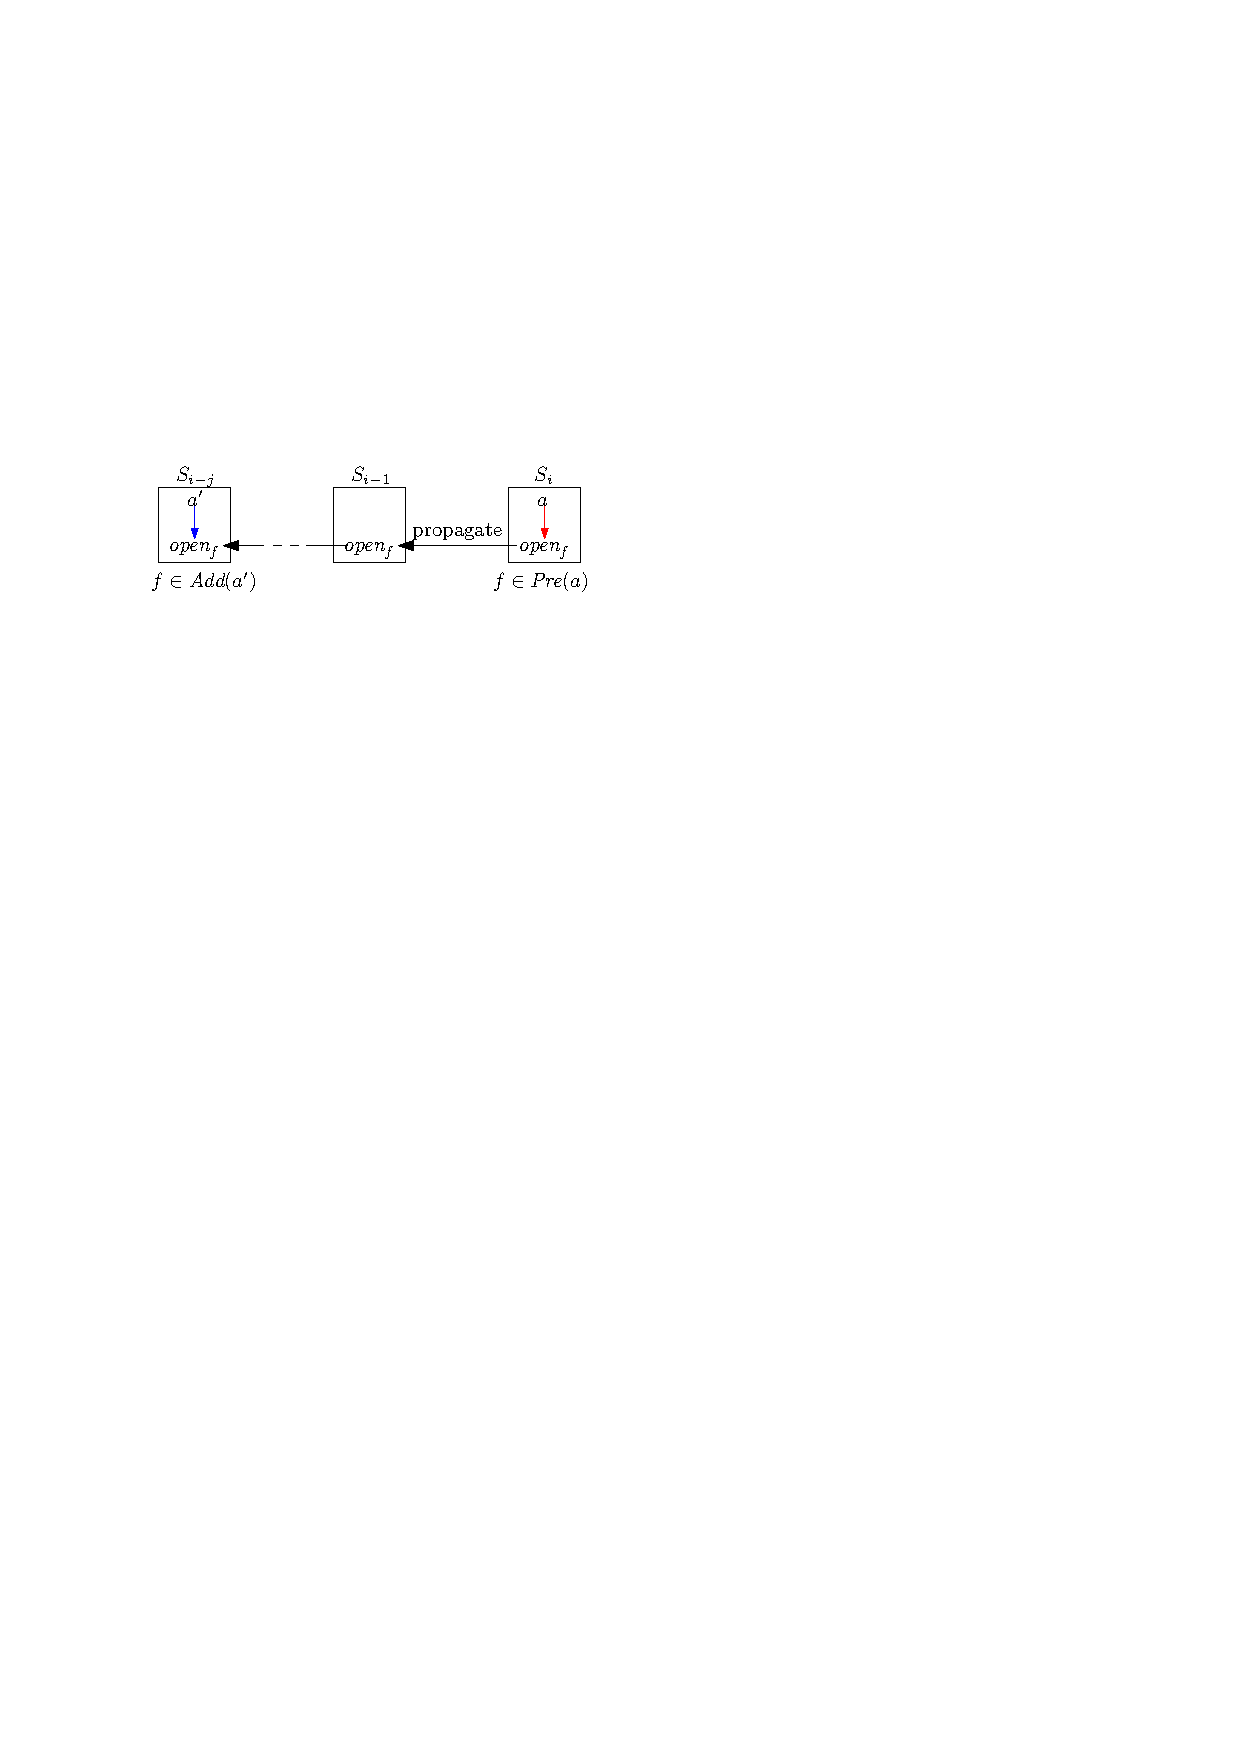
\includegraphics[width=.5\textwidth]{figures/transitions}
    \caption{Lien causal: $\b$ produit $\f$ pour $\a$.}
    \label{fig:causal-link-cte}
\end{figure}

Nous définissons l'ensemble des variables \enquote{open}, noté $\openSet$, comme $\openSet = \{\openSingle{\f} ~|~ \f \in \F \}$. Chaque action étant considérée comme une variable propositionnelle, nous définissons un ensemble de variables propositionnelles $\X$, donné par $\X = \A \cup \openSet$.


\paragraph*{[CTE-OPEN.0 -- Quantificateurs]}

Pour chaque profondeur $i$ de l'arbre, $\X_i$ dénote une copie de l'ensemble des variables $\X$ \fred{à reformuler}. Il existe une seule variable $\instepcte{\a}{i}\in X_{i}$ pour chaque action utilisée pour déterminer la dernière transition dans le plan et une seule variable $\openstepcte{\f}{i}\in X_{i}$ pour chaque fluent utilisée pour déterminer si $\f$ est une condition ouverte. A la même profondeur~$i$, la valeur de ces variables dépend du n\oe ud (correspondant à une étape du plan) sélectionné par les valeurs des variables universelles de branchement supérieures $b_{i+1}\ldots b_{\depth}$.

%\begin{small}
%\[
%\begin{matrix}
%\displaystyle \bigexists_{\a \in \A} \a_{\depth}. \bigexists_{\f\in \F} %\open{\f}{\depth}.%\\
%\displaystyle {\bigforall b_{\depth}.}\\
%\displaystyle \bigexists_{\a \in \A} \a_{\depth-1}. \bigexists_{\f\in \F} %\open{\f}{\depth-1}.%\\
%\displaystyle {\bigforall b_{\depth-1}.}\\
%\displaystyle \dots\\ 
%%\dots
%\displaystyle \bigexists_{\a \in \A} \a_{1}. \bigexists_{\f\in \F} %\open{\f}{1}.%\\
%\displaystyle {\bigforall b_{1}.}%\\
%\displaystyle \bigexists_{\a \in \A} \a_{0}. \bigexists_{\f\in \F} %\open{\f}{0}.
%\end{matrix}
%\]
%\end{small}\\

\begin{small}
\[
\begin{matrix}
\displaystyle \bigexists_{\a \in \A} \instepcte{\a}{\depth}. \bigexists_{\f\in \F} \openstepcte{\f}{\depth}.%\\
\displaystyle {\bigforall b_{\depth}.}\\
\displaystyle \bigexists_{\a \in \A} \instepcte{\a}{\depth-1}. \bigexists_{\f\in \F} \openstepcte{\f}{\depth-1}.%\\
\displaystyle {\bigforall b_{\depth-1}.}\\
\displaystyle \dots\\ 
%\dots
\displaystyle \bigexists_{\a \in \A} \instepcte{\a}{1}. \bigexists_{\f\in \F} \openstepcte{\f}{1}.%\\
\displaystyle {\bigforall b_{1}.}%\\
\displaystyle \bigexists_{\a \in \A} \instepcte{\a}{0}. \bigexists_{\f\in \F} \openstepcte{\f}{0}.
\end{matrix}
\]
\end{small}\\

%Dans ce qui suit, un \textit{n\oe ud} désigne maintenant un n\oe ud qui n'est pas une feuille. % et $\depth$ est la profondeur de l'arbre.
%Le prédécesseur d'un n\oe ud au niveau $i$ est la feuille la plus à droite du sous-arbre gauche. Le successeur d'un noeud au niveau $i$ est la feuille la plus à gauche du sous-arbre droit.
%Afin de sélectionner ces transitions, nous introduisons l'opérateur feuille-vers-n\oe ud $\leftselect{i}$ défini comme:
%%\begin{scriptsize}
%\[\leftselect{i} \equiv \neg b_{i} \wedge \BigforallTwo{j=1}{i-1} b_{j}.\]
%%\end{scriptsize}
%Symétriquement, nous introduisons l'opérateur n\oe ud-vers-feuille $\rightselect{i}$ défini comme:
%%\begin{scriptsize}
%\[\rightselect{i} \equiv b_{i} \wedge \BigforallTwo{j=1}{i-1} \neg b_{j}.\]
%%\end{scriptsize}

\paragraph*{[CTE-OPEN.1 -- Conditions ouvertes]}
%\displaystyle\mathop{\exists \a_{1}}_{\a \in \A} .\displaystyle\mathop{\exists \open{\f}{1}}_{\f\in \F} .\forall b_{1}. \displaystyle\mathop{\exists \a_{0}}_{\a \in \A} .\displaystyle\mathop{\exists \open{\f}{0}}_{\f\in \F} .\\
Si une action $\a$ est exécutée dans une étape du plan, alors chaque précondition de $\a$ doit être une condition ouverte à cette étape (c'est-à-dire qu'un lien causal est requis pour cette précondition).
%\begin{scriptsize}
%\[ \BigforallTwo{i=0}{\depth} \Bigforall{\a \in \A} \left(\a_{i} \Rightarrow \Bigforall{\f\in \Cond{\a}} \open{\f}{i}\right) \]
%\end{scriptsize}

\begin{small}
\[ \BigforallTwo{i=0}{\depth} \Bigforall{\a \in \A} \left(\instepcte{\a}{i} \Rightarrow \Bigforall{\f\in \Cond{\a}} \openstepcte{\f}{i}\right) \]
\end{small}

Dans la dernière étape du plan menant au but (c'est-à-dire la feuille la plus à droite de l'arbre), tous les fluents du but doivent être des conditions ouvertes ou ajoutées par des actions exécutées dans cette étape.
%\begin{scriptsize}
%\[ \BigforallTwo{i=1}{\depth}b_{i} \Rightarrow \Bigforall{\f\in G} \left(\open{\f}{0} \vee \bigvee\limits_{\substack{\a \in \A \\ \f \in \Add{\a}}} \a_{0}\right) \]
%\end{scriptsize}

\begin{small}
\[ \BigforallTwo{i=1}{\depth}\instepcte{b}{i} \Rightarrow \Bigforall{\f\in G} \left(\openstepcte{\f}{0} \vee \bigvee\limits_{\substack{\a \in \A \\ \f \in \Add{\a}}} \instepcte{\a}{0}\right) \]
\end{small}

\paragraph*{[CTE-OPEN.2 -- Propagation et fermeture]}

Aucune condition ne doit rester ouverte dans la première étape du plan (c'est-à-dire la feuille la plus à gauche de l'arbre) si elle n'est pas présente dans l'état initial.
%\begin{scriptsize}
%\[ \BigforallTwo{i=1}{\depth}\neg b_{i} \Rightarrow \Bigforall{\f\in \F\setminus I} \neg \open{\f}{0} \]	
%\end{scriptsize}

\begin{small}
\[ \BigforallTwo{i=1}{\depth}\neg \instepcte{b}{i} \Rightarrow \Bigforall{\f\in \F\setminus I} \neg \openstepcte{\f}{0} \]	
\end{small}

Toute condition ouverte dans une étape doit, soit rester ouverte, soit être ajoutée (fermée) par une action à l'étape précédente.

%\begin{scriptsize}
%\[ \BigforallTwo{i=1}{\depth} \Bigforall{\f\in \F} \left(\left(\open{\f}{i} \wedge \leftselect{i} \right) \Rightarrow \left(\open{\f}{0} \vee \bigvee\limits_{\substack{\a \in \A \\ \f \in \Add{\a}}} \a_{0}\right)\right) \]
%
%\[ \BigforallTwo{i=1}{\depth}\Bigforall{\f\in \F}\left(\left(\open{\f}{0} \wedge \rightselect{i} \right) \Rightarrow \left(\open{\f}{i} \vee \bigvee\limits_{\substack{\a \in \A \\ \f \in \Add{\a}}} \a_{i}\right)\right)
%\]
%\end{scriptsize}

\begin{small}
\[ \BigforallTwo{i=1}{\depth} \Bigforall{\f\in \F} \left(\left(\openstepcte{\f}{i} \wedge \leftselect{i} \right) \Rightarrow \left(\openstepcte{\f}{0} \vee \bigvee\limits_{\substack{\a \in \A \\ \f \in \Add{\a}}} \instepcte{\a}{0}\right)\right) \]

\[ \BigforallTwo{i=1}{\depth}\Bigforall{\f\in \F}\left(\left(\openstepcte{\f}{0} \wedge \rightselect{i} \right) \Rightarrow \left(\openstepcte{\f}{i} \vee \bigvee\limits_{\substack{\a \in \A \\ \f \in \Add{\a}}} \instepcte{\a}{i}\right)\right)
\]
\end{small}


 \paragraph*{[CTE-OPEN.3 -- Protection des conditions ouvertes]}

Une condition ouverte dans une étape donnée ne peut pas être supprimée à l'étape précédente. Cela garantit de ne rompre aucun lien de causalité dans le plan.
%\begin{scriptsize}
%\[ \BigforallTwo{i=1}{\depth} \Bigforall{\f\in \F}\left(\left(\open{\f}{i} \wedge \leftselect{i} \right) \Rightarrow \Bigforall{\a \in \A\\ \f \in \Del{\a}}\neg \a_{0}\right) \]
%\[ \BigforallTwo{i=1}{\depth} \Bigforall{\f \in \F} \left(\left(\open{\f}{0} \wedge \rightselect{i} \right) \Rightarrow \Bigforall{\a \in \A \\ \f \in \Del{\a}}\neg \a_{i}\right) \]
%\end{scriptsize}

\begin{small}
\[ \BigforallTwo{i=1}{\depth} \Bigforall{\f\in \F}\left(\left(\openstepcte{\f}{i} \wedge \leftselect{i} \right) \Rightarrow \Bigforall{\a \in \A\\ \f \in \Del{\a}}\neg \instepcte{\a}{0}\right) \]
\[ \BigforallTwo{i=1}{\depth} \Bigforall{\f \in \F} \left(\left(\openstepcte{\f}{0} \wedge \rightselect{i} \right) \Rightarrow \Bigforall{\a \in \A \\ \f \in \Del{\a}}\neg \instepcte{\a}{i}\right) \]
\end{small}

\paragraph*{[CTE-OPEN.4 -- Prévention des interactions négatives]}

Si une action supprime un fluent qui est nécessaire ou est ajouté par une autre action, alors ces deux actions ne peuvent pas être exécutées toutes les deux dans une même étape.
%\begin{scriptsize}
%\[ \BigforallTwo{i=0}{\depth} \Bigforall{\a \in \A} \Bigforall{\f\in \left(\Add{\a} \cup \Cond{\a}\right)} \Bigforall{\b \in \A \\ \a \neq \b \\ \f \in \Del{\b}}\left(\neg \a_{i} \vee \neg \b_{i}\right) \]
%\end{scriptsize}

\begin{small}
\[ \BigforallTwo{i=0}{\depth} \Bigforall{\a \in \A} \Bigforall{\f\in \left(\Add{\a} \cup \Cond{\a}\right)} \Bigforall{\b \in \A \\ \a \neq \b \\ \f \in \Del{\b}}\left(\neg \instepcte{\a}{i} \vee \neg \instepcte{\b}{i}\right) \]
\end{small}


%
% codage CTE-EFA
%
\subsubsection{Nouveau codage QBF dans les espaces d'états: CTE-EFA}

Dans ce codage, nous définissons l'ensemble des variables propositionnelles comme $\X = \A \cup \F$. Chaque étape est maintenant définie par une transition (comme dans CTE-OPEN) ainsi que par l'état résultant (valuation des fluents de $\F$). La formule est une adaptation au CTE des règles bien connues de codage SAT de \cite{KS92} basées sur des frame-axiomes explicatifs dans les espaces d'états.

\paragraph*{Quantificateurs}

A chaque profondeur $i$ de l'arbre, il existe une seule variable $\a_{i}$ pour chaque action utilisée pour déterminer la dernière transition dans le plan et une seule variable $\f_{i}$ pour chaque fluent utilisée pour déterminer l'état.
A la même profondeur $i$, les valeurs de ces variables dépendent du n\oe ud (correspondant à une transition dans le plan et à l'état résultant) sélectionné par les valeurs des variables universelles de branchement supérieures $b_{i+1}\ldots b_{\depth}$.

\begin{small}
\[
\begin{matrix}
\displaystyle \bigexists_{\a \in \A} \a_{\depth}. \bigexists_{\f\in \F} \f_{\depth}.%\\
\displaystyle {\bigforall b_{\depth}.}\\
\displaystyle \bigexists_{\a \in \A} \a_{\depth-1}. \bigexists_{\f\in \F} \f_{\depth-1}.%\\
\displaystyle {\bigforall b_{\depth-1}.}\\
\displaystyle \dots\\ 
%\dots
\displaystyle \bigexists_{\a \in \A} \a_{1}. \bigexists_{\f\in \F} \f_{1}.%\\
\displaystyle {\bigforall b_{1}.}%\\
\displaystyle \bigexists_{\a \in \A} \a_{0}. \bigexists_{\f\in \F} \f_{0}.
\end{matrix}
\]
\end{small}%\\

\paragraph*{But}

Dans l'état après la dernière transition du plan (c'est-à-dire la feuille la plus à droite de l'arbre), tous les fluents du but doivent être atteints.

%\begin{scriptsize}
\[ \BigforallTwo{i=1}{\depth} b_{i} \Rightarrow \Bigforall{\f\in G} {\f}_{0} \]	
%\end{scriptsize}

\paragraph*{Conditions et effets des actions}

Si une action $\a$ est exécutée dans une transition du plan, alors chaque effet de $\a$ se produit dans l'état résultant et chaque précondition de $\a$ est requise dans l'état précédent.
%\begin{scriptsize}
\[ \BigforallTwo{i=0}{\depth} \Bigforall{\a \in \A} \left(\a_{i} \Rightarrow \left( \Bigforall{\f\in \Add{\a}} \f_{i} \right) \wedge \left( \Bigforall{\f\in \Del{\a}} \neg \f_{i} \right) \right) \]
%\end{scriptsize}

%\begin{scriptsize}
\[ \BigforallTwo{i=1}{\depth} \Bigforall{\a\in \A}
\left(\a_{i} \wedge \leftselect{i} \Rightarrow \Bigforall{\f \in \Cond{\A}} \f_{0}\right)\]
\[\BigforallTwo{i=1}{\depth} \Bigforall{\a\in \A}
\left(\a_{0} \wedge \rightselect{i} \Rightarrow \Bigforall{\f \in \Cond{\A}} \f_{i}\right)\]
%\end{scriptsize}

De plus, une action qui n'a pas toutes ses préconditions dans l'état initial ne peut pas être exécutée dans la première transition du plan (c'est-à-dire la feuille la plus à gauche de l'arbre):

%\begin{scriptsize}
\[ \BigforallTwo{i=1}{\depth}\neg b_{i} \Rightarrow \Bigforall{\a\in \A\\ \Cond{\a} \not\subset I} \neg {\a}_{0} \]
%\end{scriptsize}

\paragraph*{Frame-axiomes explicatifs}

%{\color{blue}We only give here one of the four rules for explanatory frame axioms, the others being very similar. \color{red} Fred: j'ai ajouté les 4 règles + celles pour l'étape initiale}
Si la valeur d'un fluent change entre deux états consécutifs, alors une action qui produit cette modification est exécutée dans la transition du plan entre ces états.

\begin{small}
\[ \BigforallTwo{i=1}{\depth} \Bigforall{\f\in \F}
\left(\left(\neg\f_{0} \wedge \f_{i} \wedge \leftselect{i} \right) \Rightarrow \left(\bigvee\limits_{\substack{\a \in \A \\ \f \in \Add{\a}}} \a_{i}\right)\right)\]

\[ \BigforallTwo{i=1}{\depth} \Bigforall{\f\in \F}
\left(\left(\neg\f_{i} \wedge \f_{0} \wedge \rightselect{i} \right) \Rightarrow \left(\bigvee\limits_{\substack{\a \in \A \\ \f \in \Add{\a}}} \a_{0}\right)\right)\]
\end{small}

\begin{small}
\[ \BigforallTwo{i=1}{\depth} \Bigforall{\f\in \F}
\left(\left(\f_{0} \wedge \neg\f_{i} \wedge \leftselect{i} \right) \Rightarrow \left(\bigvee\limits_{\substack{\a \in \A \\ \f \in \Del{\a}}} \a_{i}\right)\right)\]
\[ \BigforallTwo{i=1}{\depth} \Bigforall{\f\in \F}
\left(\left(\f_{i} \wedge \neg\f_{0} \wedge \rightselect{i} \right) \Rightarrow \left(\bigvee\limits_{\substack{\a \in \A \\ \f \in \Del{\a}}} \a_{0}\right)\right)\]
\end{small}

Une règle supplémentaire est également requise pour décrire les frame-axiomes explicatifs pour la première transition du plan à partir de l'état initial (c'est-à-dire la feuille la plus à gauche de l'arbre):

%\begin{scriptsize}
\[ \Bigforall{\f\in \F\setminus I} \left(\left(\f_{0}\wedge \BigforallTwo{i=1}{\depth}\neg b_{i}\right) \Rightarrow \Bigexists{\a\in \A\\ \f\in\Add{\a}\\\Cond{\a} \subset I} {\a}_{0} \right) \]
\[ \Bigforall{\f\in I} \left(\left(\neg\f_{0}\wedge \BigforallTwo{i=1}{\depth}\neg b_{i}\right) \Rightarrow \Bigexists{\a\in \A\\ \f\in\Del{\a}\\\Cond{\a} \subset I} {\a}_{0} \right) \]
%\end{scriptsize}

\paragraph*{Prévention des interactions négatives}

Contrairement à CTE-NOOP et CTE-OPEN, les effets contradictoires sont déjà interdits par les règles précédentes (effets des actions).
Cette règle doit donc seulement empêcher les interactions entre les préconditions et les retraits des actions. Si une action supprime un fluent nécessaire à une autre action, ces deux actions ne peuvent pas être exécutées dans une même transition du plan.

%\begin{scriptsize}
\[ \BigforallTwo{i=0}{\depth} \Bigforall{\a \in \A} \Bigforall{\f\in \Cond{\a}} \Bigforall{\b \in \A \\ \a \neq \b \\ \f \in \Del{\b}}\left(\neg \a_{i} \vee \neg \b_{i}\right) \]
%\end{scriptsize}



%\subsection{Finding Minimal Plan Length}

%\begin{figure}[ht]
%\begin{center} \includegraphics[width=.45\textwidth]{images/dichotomie-1} \end{center}
%\caption{incremental search}
%\end{figure}






%%%%%%%%%%%%%%%%%%%%%%%%%%%%%
% PLANIFICATION SMT
%%%%%%%%%%%%%%%%%%%%%%%%%%%%%
\section{Planification temporelle SMT}
%


%\subsection{Planification temporelle}
\subsection{Définitions préliminaires}

%Nous étudions la planification temporelle propositionnelle dans un langage basé sur les aspects temporels de PDDL2.1 \cite{DBLP:journals/jair/FoxL03}. 
Un fluent est une proposition atomique positive ou négative. Comme dans PDDL2.1, nous considérons que les changements des valeurs des fluents sont instantanés mais que les conditions sur la valeur des fluents peuvent être imposées sur un intervalle. Une action $\a$ est un quadruplet $\langle\cond{\a},\add{\a},\del{\a},\constr{a}\rangle$, où l'ensemble des conditions $\cond{\a}$ est l'ensemble des fluents qui doivent être vrais pour que $\a$ soit exécutée, l'ensemble des ajouts $\add{\a}$ est l'ensemble des fluents qui sont établis par $\a$, l'ensemble des retraits $\del{\a}$ est l'ensemble des fluents qui sont détruits par $\a$, et l'ensemble de contraintes $\constr{a}$ est un ensemble de contraintes entre les temps relatifs des événements qui se produisent pendant l'exécution de $\a$. Un événement correspond à l'une des quatre possibilités: l'établissement ou la destruction d'un fluent par une action $\a$, ou le début ou la fin d'un intervalle sur lequel un fluent est requis par une action $\a$. Dans PDDL2.1, les événements ne peuvent se produire qu'au début ou à la fin des actions, mais nous rel\^{a}chons cette hypothèse de sorte que les événements peuvent se produire à tout moment à condition que les contraintes $\constr{\a}$ soient satisfaites. Notons que $\add{\a} \cap \del{\a}$ peut être non vide. En effet, il n'est pas inhabituel pour une action durative d'établir un fluent au début de l'action et de le détruire à sa fin. Nous pouvons également observer que la durée d'une action, le temps entre le premier et le dernier événement de l'action, n'a pas besoin d'être explicitement stockée.
%Nous représentons des actions non-instantanées par un rectangle. La durée d'une action est donnée entre crochets après le nom de l'action. Les conditions sont écrites au-dessus d'une action, et les effets ci-dessous. L'action CHARGE (m, c) représentée sur la figure 1 représente le chargement d'un lot de béton c dans un mélangeur m. Nous avons Cond (LOAD (m, c)) = {Fluid (c), Empty (m), At-factory (m)}. On peut voir sur la figure que le mélangeur doit être vide au début du chargement, alors que le béton doit être fluide et le malaxeur à l'usine pendant toute la durée du chargement. Nous avons Del (LOAD (m, c)) = {Empty (m)} et Add (LOAD (m, c) = {On (m, c)} Nous pouvons voir sur la figure que dès que le chargement commence, le mélangeur n'est plus vide et à la fin du chargement le mélangeur contient le béton.


Nous utilisons la notation $\a \rightarrow \f$ pour désigner l'événement que l'action $\a$ établit le fluent $\f$, $\a \rightarrow \neg\f$ pour désigner l'événement que $\a$ détruit $\f$, et $\f \mid\rightarrow \a$ et $\f \rightarrow\mid \a$, respectivement, pour indiquer le début et la fin de l'intervalle sur lequel $\a$ requiert la condition $\f.$ Si $\f$ est déjà vrai (respectivement, faux) lorsque l'événement
$\a \rightarrow \f$ ($\a \rightarrow \neg\f$) se produit, nous considérons toujours que $\a$ établit (détruit) $\f$. Un plan temporel peut contenir plusieurs instances de la même action, mais %puisque la plupart des plans temporels étudiés dans cet article contiennent au plus un exemple de chaque action, 
par simplicité de notation, nous ferons seulement la distinction entre actions et instances d'action si cela est absolument nécessaire. Nous utilisons la notation $\tau(e)$ pour représenter l'instant dans un plan où un événement $e$ se produit.
Pour une action donnée (ou une instance d'action) $a$, $\events{\a}$ représente les différents événements qui constituent sa définition, à savoir $\a \rightarrow \f$ pour tout $\f$ dans $\add{\a}$, $\a \rightarrow \neg\f$ pour tout $\f$ dans $\del{\a}$, $\f \mid\rightarrow \a$ et $\f \rightarrow\mid \a$ pour tout $\f$ dans $\cond{a}$. La définition d'une action $\a$ inclut les contraintes $\constr{a}$ sur les instants relatifs aux événements dans $\events{\a}$. %Par exemple, la structure interne de l'action de longueur fixe LOAD (m, c) représentée sur la figure 1 est définie par des contraintes telles que
%τ (Fluide (c) → | CHARGE (m, c)) - τ (Fluide (c) | → CHARGE (m, c)) = 5
%τ (LOAD (m, c) → On (m, c)) - τ (Fluide (c) → | LOAD (m, c)) = 0
Comme dans PDDL2.1, nous considérons que la durée entre événements dans $\events{\a}$ n'est pas nécessairement fixe et que $\constr{\a}$ est un ensemble de contraintes d'intervalle sur des paires d'événements, tels que
$\tau(\f \rightarrow\mid \a) - \tau(\f \mid\rightarrow \a) \in [\alpha,\beta]$ pour des constantes $\alpha,\beta$. Nous utilisons $[\alpha_{\a}(e_1, e_2), \beta_{\a}(e_1, e_2)]$ pour désigner l'intervalle de valeurs possibles pour la distance relative entre les événements $e_1$, $e_2$ de l'action $\a$. Une durée fixe entre les événements $e_1,e_2 \in \events{\a}$ peut, bien s\^{u}r, être modélisée en définissant $\alpha_{\a}(e_1, e_2)=\beta_{\a}(e_1, e_2)$. De même, l'absence de contrainte peut être modélisée par l'intervalle $[-\infty,+\infty]$. Nous introduisons maintenant deux contraintes fondamentales que tous les plans temporels doivent satisfaire :
\begin{itemize}
\item les \emph{contraintes inhérentes} à l'ensemble des instances d'action $\A$ : pour toute $\a\in\A$, $\a$ satisfait $\constr{a}$, c'est-à-dire pour toutes les paires d'événements $e_1,e_2\in \events{\a}$ nous avons $\tau(e_1) - \tau(e_2) \in [\alpha_\a(e_1,e_2),\beta_\a(e_1,e_2)]$ ;
\item les \emph{contraintes d'effets contradictoires} sur l'ensemble des instances d'action $\A$ : pour toutes $\a_i,\a_j \in\A$, pour tout fluent positif $\f \in \del{\a_i} \cap \add{\a_j}$ nous avons $\tau(\a_i \rightarrow \neg\f) \neq \tau(\a_j \rightarrow \f)$.
\end{itemize}

Les contraintes inhérentes définissent la structure interne de chaque instance d'action, alors que les contraintes d'effets contradictoires assurent que la valeur de vérité de chaque fluent ne soit jamais indéfinie lors de l'exécution d'un plan temporel. %Par exemple, si un plan contient une instance $\a$ de l'action LOAD (m, c) montrée à la figure 1 et une instance b d'une autre action CLEAN (m) avec Empty (m) ∈ Add (CLEAN (m)), alors le plan temporel doit satisfaire la contrainte d'effets contradictoires
%τ (a → ¬EMPTY (m)) ≠ τ (b → EMPTY (m)).

\begin{definition}
Un problème de planification temporelle $\langle \I, \A, \G \rangle$ consiste en un ensemble d'actions $\A,$ un état initial $\I$ et un but $\G$, où $\I$ et $\G$ sont des ensembles de fluents.
\end{definition}
\paragraph*{Notation} Si $\A$ est un ensemble d'instances d'actions, alors $\events{\A}$ est l'union des ensembles $\events{\a}$ (pour toutes les instances d'action $a\in \A$).

\begin{definition}\label{def:plan-temporel}
$P = \langle \A, \tau \rangle$, où $\A$ est un ensemble fini d'instances d'actions $\{a_1,\ldots, a_n\}$ et $\tau$ est une fonction à valeurs réelles sur $\events{\A}$, est un plan temporel pour le problème $\langle \I , \A^{\prime}, \G \rangle$ si
\begin{enumerate}
\item[(1)] $\A \subseteq \A^{\prime}$, et
\item[(2)] $P$ vérifie les contraintes inhérentes et contradictoires sur $\A$;
\end{enumerate}
et lorsque $P$ est exécuté (c'est-à-dire que les fluents sont établis ou détruits aux instants donnés par $\tau$) à partir de l'état initial $\I$:
\begin{enumerate}
\item[(3)] pour toute $a_i \in \A$, chaque $\f \in \cond{a_i}$ est vrai lorsqu'il est requis, et
\item[(4)] tous les fluents $g \in \G$ sont vrais à la fin de l'exécution de $P$.
\item[(5)] $P$ est robuste sous des changements infinitésimaux dans les temps de démarrage des actions.
\end{enumerate}
\end{definition}

Les événements sont instantanés, alors que les actions ont non seulement une durée mais celle-ci peut aussi être de longueur variable. Ainsi, un plan temporel $P$ ne planifie pas directement ses instances d'action mais planifie tous les événements dans ses instances d'actions.
La condition (5) de la définition~\ref{def:plan-temporel} signifie que nous interdisons les plans qui exigent une synchronisation parfaite entre différentes actions. % montrent comment 
Cette condition peut être imposée dans PDDL2.1 \cite{DBLP:conf/ecai/FoxLH04}. Nous exigeons que dans tous les plans, les fluents soient établis strictement avant le début de l'intervalle sur lequel ils sont requis. La seule exception à cette règle est lorsqu'un fluent $\f$ est établi et requis par la même action $\a$. Nous permettons la possibilité d'une parfaite synchronisation au sein d'une action, ce qui signifie que nous pouvons avoir $\tau(\a\rightarrow\f)=\tau(\f\mid\rightarrow\a)$.
De même, les fluents ne peuvent être détruits qu'après la fin de l'intervalle sur lequel ils sont requis. La seule exception à cette regle est quand un fluent $\f$ est requis et détruit par une action $\a$, auquel cas on peut avoir $\tau(\f\rightarrow\mid\a)=\tau(\a\rightarrow\neg\f)$. %Par exemple, le fluide Empty (m) est simultanément requis et détruit par l'action LOAD (m, c) représentée sur la figure 1.

\begin{definition}
Un problème de planification temporelle $\langle \I, \A, \G \rangle$ est positif s'il n'y a pas de fluents négatifs dans les conditions d'actions ni dans le but $\G$.
\end{definition}

Dans cet article, nous ne considèrerons que des problèmes de planification temporelle positifs $\langle \I, \A, \G \rangle$. Il est bien connu que tout problème de planification peut être transformé en un problème positif équivalent en temps linéaire par l'introduction, pour chaque fluent positif $\f$, d'un nouveau fluent pour remplacer les occurrences de $\neg\f$ dans les conditions d'actions \cite{DBLP:books/daglib/0014222}. %Il est important de noter, cependant, que cette transformation peut ne pas conserver d'autres propriétés de l'instance. 
En supposant que tous les problèmes sont positifs, $\G$ et $\cond{\a}$ (pour toute action $\a$) sont composés de fluents positifs. Par convention, $\add{\a}$ et $\del{a}$ sont aussi composés exclusivement de fluents positifs. L'état initial $\I$, cependant, peut contenir des fluents négatifs.
%Pour simplifier la présentation, nous supposons dans cet article que l'ensemble des actions A a subi l'opération de filtrage consistant à éliminer les actions $\a$ de $\A$ qui ne peuvent être exécutées puisque $\cond{\a}$ n'est pas un sous-ensemble de $\I\cup\add{\a}$.


%\subsubsection{Codage SAT pour la planification classique}
%Dans cette section, nous considérons la planification classique comme restriction de la planification temporelle décrite dans la section précédente. Un problème de planification positif est donc ici un triplet $\langle \I , \A, \G \rangle$ tel que toutes les actions de $\A$ sont instantanées (c'est-à-dire $\forall \a\in\A, \forall e_1,e_2\in \events{\a}, \tau(e_1)=\tau(e_2)$). De plus, nous considérons pour tout plan $P = \langle \A, \tau \rangle$, que $\tau$ est une fonction à valeurs entières de $\events{\A}$ dans $N=\{1,\ldots,n\}$ l'ensemble ordonné des index d'étapes de $P$.


%
% codage-open-sat (old)
%
%





%\begin{frame}
%\begin{figure}\label{steps}
% \hspace{0.8em}\xymatrix@C=1pc@R=1pc{
%  Init \ar[r] & \fbox{S$_{1}$} \ar[r]  & \fbox{S$_{2}$} \ar[r] & \fbox{S$_{3}$} \ar[r] & \fbox{S$_{4}$} \ar[r] & \fbox{S$_{5}$} \ar[r] & \fbox{S$_{6}$} \ar[r] & \fbox{S$_{7}$} \ar[r] & Goal \\
%  }
%  \vspace{2em}
%   \hspace{0.8em}\xymatrix@C=0.2pc@R=1pc{
%   & & & & & \fbox{S$_{4}$} \ar@{.}[lld] \ar@{.}[rrd] \ar@/^1pc/[rdd] \\
%   & & & \fbox{S$_{2}$} \ar[rd] & & & & \fbox{S$_{6}$} \ar[rd] \\
%  Init \ar[rr] & & \fbox{S$_{1}$} \ar[ru]  & & \fbox{S$_{3}$} \ar@/^1pc/[ruu] & & \fbox{S$_{5}$} \ar[ru] & & \fbox{S$_{7}$} \ar[rr] & & Goal \\
%  }
%\caption{Transitions of an 8-steps plan in SAT/SMT encoding and QBF compact tree encoding (CTE)}
%\end{figure}
%\end{frame}


\subsection{Codages SMT de référence pour la planification temporelle}
%

%
% SMT TLP-GP
%

\fred{Règles de TLP-GP (Maris, Régnier 2008)}

\paragraph*{Etat initial et But}

Les nœuds d'actions factices Init (produisant l'état initial) et Goal (nécessitant le but) sont tous deux vrais.

\paragraph*{Production des préconditions par liens causaux}

Si une action $\a_{i}$ est active dans le plan à une étape $i$, alors pour chacune de ses préconditions $\f$, il existe au moins un lien causal (noté $\Link{\b_{j}}{\f}{\a_{i}}$) d'une action $\b_{j}$, qui produit cette précondition à l'étape $j$, vers $\a_{i}$.

\[ \BigforallTwo{i=1}{i=\length} \Bigforall{\a\in\A} \left( \a_{i} \Rightarrow \Bigforall{\f\in\Cond{\a}} \BigexistsTwo{j=1}{j=i}\Bigexists{\b\in\A\\\f\in\Add{\b}} \Link{\b_{j}}{\f}{\a_{i}} \right)
\]

\paragraph*{Activation des actions et ordre partiel}

S’il existe un lien causal entre une action $\b_{j}$ qui produit une précondition $\f$ pour une action $\a_{i}$, alors $\b_{j}$ et $\a_{i}$ sont actives dans le plan et l’instant où $\b_{j}$ produit certainement $\f$ est antérieur ou égal à l’instant où $\a_{j}$ commence à nécessiter $\f$.

\[
\begin{matrix}
\BigforallTwo{i=1}{i=\length} \BigforallTwo{j=1}{i=j} \Bigforall{(\a,\b)\in\A^{2}} \Bigforall{\f\in\left(\Cond{\a}\cap\Add{\b}\right)}\\ \left( \Link{\b_{j}}{\f}{\a_{i}} \Rightarrow \left( \b_{j} \wedge \a_{i} \wedge \tau(\b_{j}\rightarrow\f) \leq \tau(\f\mid\rightarrow\a_{i}) \right) \right)
\end{matrix}
\]

\paragraph*{Protection des liens causaux}

Si un lien causal assure la protection d’un fluent $\f$ et qu'une action qui le détruit est active dans le plan, alors l’intervalle temporel correspondant au lien causal et l’intervalle temporel correspondant à l’activation de $\neg \f$ (la destruction de $\f$) par l’action sont disjoints.

\[
\begin{matrix}
\BigforallTwo{i=1}{i=\length} \BigforallTwo{j=1}{i=j} \BigforallTwo{k=1}{k=\length} \Bigforall{(\a,\b)\in\A^{2}} \Bigforall{\f\in\left(\Cond{\a}\cap\Add{\b}\right)} \Bigforall{\c\in\A\\\f\in\Del{\c}}\\ \left( \Link{\b_{j}}{\f}{\a_{i}} \wedge \c_{k} \Rightarrow \left( \begin{matrix} \tau(\c_{k}\rightarrow\neg\f) < \tau(\b_{j}\rightarrow\f)\\ \vee \tau(\f\rightarrow\mid\a_{i}) < \tau(\c_{k}\rightarrow\neg\f) \end{matrix} \right) \right)
\end{matrix}
\]

\paragraph*{Prévention des interactions négatives}

Si deux actions produisant respectivement une proposition p et sa négation sont actives dans le plan, alors les intervalles temporels correspondants à l’activation de p et à l’activation de ¬p sont disjoints.

\[
\begin{matrix}
\BigforallTwo{i=1}{i=\length} \BigforallTwo{j=1}{j=\length} \Bigforall{(\a,\b)\in\A^{2}} \Bigforall{\f\in\left(\Add{\a}\cap\Del{\b}\right)}\\ \left( \a_{i} \wedge \b_{j} \Rightarrow \left( \begin{matrix} \tau(\a_{i}\rightarrow\neg\f) < \tau(\b_{j}\rightarrow\f)%\\ \vee \tau(\f\rightarrow\mid\a_{i}) < \tau(\c_{k}\rightarrow\neg\f) 
\end{matrix} \right) \right)
\end{matrix}
\]

\paragraph*{Bornes inférieure et supérieure}

L’instant initial où les propositions de l’état initial sont vraies est antérieur à tous les instants de début des préconditions des actions du plan. L’instant final où les propositions du but sont vraies est postérieur à tous les instants de fin des effets des actions du plan.
\fred{à ajouter}


\subsection{Nouveau codage SMT pour la planification temporelle}

Nous introduisons une adaptation SMT du codage SAT basé sur les conditions ouvertes que nous avons introduit dans la section \fred{ajout référence} pour la planification classique. Ici, les actions ne sont plus instantanées et des contraintes sur les instants $\tau(e)$ auxquels se produisent des événements $e\in\events{\A}$ doivent explicitement être ajoutées.


Considérons donc maintenant un problème de planification temporelle positif $\langle \I, \A, \G \rangle$.
Pour chaque instance d'action $\a$ et chaque fluent $\f\in \cond{a}$, nous introduisons deux variables $\tau_{s}(\textit{open}_{f})$ et $\tau_{e}(\textit{open}_{f})$ qui nous permettent de définir un intervalle temporel de protection de lien causal depuis l'état initial ou une étape contenant une action qui produit $\f$ vers une étape qui contient l'instance d'action $\a$. Durant cet intervalle temporel, aucune action ne pourra détruire $\f$.


%%\paragraph*{Planning with Continuous Time}
%%%\begin{alertblock}{Definition}
%%For each action $a = \langle \cond{a},\add{a},\del{a} \rangle$:
%%\begin{itemize}
%%  \item $\forall f\in \cond{a}$ we define:
%%    \begin{itemize}
%%      \item $[\tau(f\mid\rightarrow a);\tau(f\rightarrow\mid a)]$
%%%      \item $open_{f}$
%%      \item $[\tau_{s}(\textit{open}_{f});\tau_{e}(\textit{open}_{f})]$
%%    \end{itemize}
%%  \item $\forall f\in \add{a}$ we define $[\tau(a\mid\rightarrow f);\tau(a\rightarrow\mid f)]$
%%  \item $\forall f\in \del{a}$ we define $[\tau(a\mid\rightarrow \neg f);\tau(a\rightarrow\mid \neg f)]$
%%\end{itemize}
%%%\begin{itemize}
%%%  \item $A \wedge (f\in \cond{A}) \rightarrow f_{~[\tau(f\mid\rightarrow A);\tau(f\rightarrow\mid A)]}$
%%%  \item $A \wedge (f\in \add{A}) \rightarrow f_{~[\tau(A\mid\rightarrow f);\tau(A\rightarrow\mid f)]}$
%%%  \item $A \wedge (f\in \del{A}) \rightarrow \neg f_{~[\tau(A\mid\rightarrow \neg f);\tau(A\rightarrow\mid \neg f)]}$
%%%\end{itemize}
%%%\end{alertblock}


%\begin{frame}{SMT Temporal Planning}
%Classical planning: PSPACE-complete~\cite{DBLP:journals/ai/Bylander94}.
%\end{frame}


\paragraph*{Conditions ouvertes} Si une action $\a$ est exécutée dans une étape du plan, alors chaque condition de $\a$ doit être une condition ouverte à cette étape (c'est-à-dire qu'un lien causal est requis pour cette condition). De plus, le début de l'intervalle sur lequel cette condition est requise se trouve dans l'intervalle de protection du lien causal $[\tau_{s}(\textit{open}_{f});\tau_{e}(\textit{open}_{f})]$.

\begin{small}
\[
%\begin{multline*}
%~\\[-3em]
\BigforallTwo{i=1}{\length}\bigwedge\limits_{\substack{\a\in \A}}%\hfill\\
\left(\a_{i} \Rightarrow \Bigforall{\substack{\f\in \cond{\a}}}\begin{pmatrix}\open{\f}{i}\hfill\\ \wedge \left(\tau(\f\mid\rightarrow\a_{i}) \geq \tau_{s}(\open{\f}{i})\right)\hfill\\
 \wedge \left(\tau(\f\mid\rightarrow\a_{i}) \leq \tau_{e}(\open{\f}{i})\right)\end{pmatrix}\right)%\hfill\\[-2em]
%%%
%\end{multline*}
\]
\end{small}

Dans la dernière étape du plan menant au but tous les fluents du but doivent être des conditions ouvertes ou ajoutées par des actions exécutées dans cette étape. Dans le cas où une action $\a$ ajoute une condition ouverte $\f$, le début de l'intervalle de protection du lien causal correspondant est fixé à l'instant où $\a$ produit $\f$.

\begin{small}
\[
%\begin{multline*}
%~\\[-3em]
\Bigforall{\substack{\f\in \G}}\begin{pmatrix}\open{\f}{\length} %\hfill\\
\vee \Bigexists{\substack{\a\in \A\\\f \in \add{\a}}}\begin{pmatrix}\a_{\length}\hfill\\
 \wedge \left(\tau(\a_{\length}\rightarrow \f) = \tau_{s}(\open{\f}{\length})\right)\hfill\\
  \wedge \left(\tau_{\mathit{Goal}} = \tau_{e}(\open{\f}{\length})\right)\hfill\end{pmatrix}\end{pmatrix}\hfill\\[-2em]
%
%\bigwedge\limits_{\substack{\mathbf{f}\in \mathbf{G}}}\left(\tau_{\textit{Goal}} = \tau_{e}(open_{\mathbf{f},\mathbf{length}})\right)\hfill\
%%%
%\end{multline*}
\]
\end{small}


\paragraph*{Propagation et fermeture}

Aucune condition ne doit rester ouverte dans la première étape du plan si elle n'est pas fournie dans l'état initial.

\begin{small}
\[
%\begin{multline*}
%~\\[-3em]
\Bigforall{\substack{\f\in \F\setminus \I}}\neg \open{\f}{1}%\hfill\\[-2em]
%%%
%\end{multline*}
\]
\end{small}

Si une condition ouverte est fournie par l'état initial, alors le début de l'intervalle de protection du lien causal correspondant est fixé à l'instant initial $\tau_{\textit{Init}}$.

\begin{small}
\[
%\begin{multline*}
%~\\[-3em]
\Bigforall{\substack{\f\in \I}}\left(\open{\f}{1} \Rightarrow \left(\tau_{\mathit{Init}} = \tau_{s}(\open{\f}{1})\right)\right)%\hfill\\[-2em]
%%%
%\end{multline*}
\]
\end{small}

Toute condition ouverte $\f$ dans une étape doit à l'étape précédente : (1) soit rester ouverte et dans ce cas l'intervalle de protection du lien causal correspondant reste le même pour ces deux étapes, (2) soit être ajoutée (fermée) par une instance d'action $\a$ et dans ce cas le début de l'intervalle de protection du lien causal est fixé à l'instant de production de $\f$ par $\a$.

\begin{small}
\[
%\begin{multline*}
%~\\[-3em]
\BigforallTwo{i=2}{\length}~\Bigforall{\substack{\f\in \F}}%\hfill\\
\begin{pmatrix}\open{\f}{i} \Rightarrow%\hfill\\
\begin{pmatrix}\begin{pmatrix}\open{\f}{i-1}\hfill\\ \wedge %\begin{pmatrix}
\left(\tau_{s}(\open{\f}{i-1}) = \tau_{s}(\open{\f}{i})\right)\hfill\\
 \wedge \left(\tau_{e}(\open{\f}{i-1}) = \tau_{e}(\open{\f}{i})
 \right)\end{pmatrix}\hfill\\
 \vee \bigvee\limits_{\substack{\a\in \A\\\f \in \add{\a}}}\left(\a_{i - 1} \wedge \left(\tau(\a_{i - 1}\rightarrow \f) = \tau_{s}(\open{\f}{i})\right)\right)\hfill\\
 \end{pmatrix}\end{pmatrix}%\\[-2em]
%%%
\]
%\end{multline*}
\end{small}


\paragraph*{Protection des conditions ouvertes}

Une condition ouverte dans une étape donnée ne peut pas être supprimée à l'intérieur de l'intervalle de protection du lien causal correspondant $[\tau_{s}(\textit{open}_{f});\tau_{e}(\textit{open}_{f})]$. Cela garantit de ne rompre aucun lien de causalité dans le plan.

\begin{small}
\[
%\begin{multline*}
%~\\[-3em]
\BigforallTwo{i=1}{\length}\BigforallTwo{j=1}{\length}%~\bigwedge\limits_{\substack{\mathbf{j}\in [1..\mathbf{\length}]}}
~\Bigforall{\substack{\f\in \F}}~\Bigforall{\substack{\a\in \A\\\f \in \del{\a}}}\hfill\\
\left(\left(\open{\f}{i} \wedge \a_{j}\right) \Rightarrow \begin{pmatrix}\left(\tau(\a_{j}\rightarrow \neg \f) < \tau_{s}(\open{\f}{i})\right)\hfill\\
 \vee \left(\tau_{e}(\open{\f}{i}) < \tau(\a_j\rightarrow \neg \f)\right)\end{pmatrix}\right)%\hfill\\[-2em]
%%%
\]
%\end{multline*}
\end{small}


\paragraph*{Prévention des interactions négatives}

Si une action $\b$ supprime, à un instant $\tau(\b\rightarrow\neg\f)$, un fluent $\f$ qui est ajouté par une autre action $\a$ à un instant $\tau(\a\rightarrow\f)$, alors ces deux instants sont différents.

\begin{small}
\[
%\begin{multline*}
%~\\[-3em]
\BigforallTwo{i=1}{\length}\BigforallTwo{j=1}{\length}%~\bigwedge\limits_{\substack{\mathbf{j}\in [1..\mathbf{\length}]}}
~\Bigforall{\substack{\a\in \A}}~\Bigforall{\substack{\f\in \add{\a}}}~\Bigforall{\substack{\b\in \A\\((i \neq j) \vee (\a \neq \b)) \wedge \f \in \del{\b}}}\hfill\\
\left(\left(\a_{i} \wedge \b_{j}\right) \Rightarrow %\begin{pmatrix}
\left(\tau(\a_{i}\rightarrow \f) \neq \tau(\b_{j}\rightarrow \neg \f)\right)%\hfill%\\
% \vee \left(\tau(\mathbf{\b}_\mathbf{j}\rightarrow\mid \neg \mathbf{\f}) < \tau(\mathbf{\a}_\mathbf{i}\mid\rightarrow \mathbf{\f})\right)
%\end{pmatrix}
\right)%\hfill\\[-2em]
%%%%%%%%%%
%\end{multline*}
\]
\end{small}

De même, si une action $\b$ supprime, à un instant $\tau(\b\rightarrow\neg\f)$, un fluent $\f$ qui est nécessaire à une autre action $\a$ sur un intervalle temporel $[\tau(\f\mid\rightarrow\a), \tau(\f\rightarrow\mid\a)]$, alors cet instant ne peut être contenu dans cet intervalle.

\begin{small}
\[
%\begin{multline*}
%~\\[-3em]
\begin{matrix}
\BigforallTwo{i=1}{\length}\BigforallTwo{j=1}{\length}%~\bigwedge\limits_{\substack{\mathbf{j}\in [1..\mathbf{\length}]}}
~\Bigforall{\substack{\a\in \A}}~\Bigforall{\substack{\f\in \cond{\a}}}~\Bigforall{\substack{\b\in \A\\((i \neq j) \vee (\a \neq \b)) \wedge \f \in \del{\b}}}\hfill\\
\left(\left(\a_{i} \wedge \b_{j}\right) \Rightarrow \begin{pmatrix}\left(\tau(\f\rightarrow\mid\a_{i}) < \tau(\b_{j}\rightarrow \neg \f)\right)\hfill\\
 \vee \left(\tau(\b_{j}\rightarrow \neg \f) < \tau(\f\mid\rightarrow\a_{i})\right)\end{pmatrix}\right)%\hfill\\[-2em]
\end{matrix}
%%%
%\end{multline*}
\]
\end{small}


%\paragraph*{SMT Encoding: bound the plan with Init and Goal states}
\paragraph*{Bornes du plan temporel}
Enfin, nous devons ajouter une contrainte pour maintenir le plan dans un intervalle de temps borné par l'étape initiale qui produit l'état initial $\I$ et l'étape finale qui nécessite tous les fluents du but $\G$.
\begin{small}
\[
%\begin{multline*}
%~\\[-2em]
\BigforallTwo{i=1}{\length}~\Bigforall{\substack{\a\in \A}}%\hfill\\
\left(\a_{i} \Rightarrow \begin{pmatrix}\Bigforall{\substack{\f\in \cond{\a}}} \begin{pmatrix}\left(\tau_{\mathit{Init}} \leq \tau(\f\mid\rightarrow\a_{i}) \right)%\hfill\\%
 \wedge \left(\tau_{\mathit{Goal}} \geq \tau(\f\rightarrow\mid\a_{i})\right) \end{pmatrix}\hfill\\
 \wedge \Bigforall{\substack{\f\in \add{\a}}} \begin{pmatrix}\left(\tau_{\mathit{Init}} \leq \tau(\a_{i}\rightarrow \f) \right)%\hfill\\%
 \wedge \left(\tau_{\mathit{Goal}} \geq \tau(\a_{i}\rightarrow \f)\right) \end{pmatrix}\hfill\\
 \wedge \Bigforall{\substack{\f\in \del{\a}}} \begin{pmatrix}\left(\tau_{\mathit{Init}} \leq \tau(\a_{i}\rightarrow \neg \f) \right)%\hfill\\%
 \wedge \left(\tau_{\mathit{Goal}} \geq \tau(\a_{i}\rightarrow \neg \f)\right) \end{pmatrix} \end{pmatrix}\right)%\\[1em]
 %%%
% \bigwedge\limits_{\substack{\mathbf{i}\in [1..\mathbf{length}]}}\bigwedge\limits_{\substack{\mathbf{A}\in \mathbf{O}}} \left(\neg \mathbf{A}_{\mathbf{i}} \Rightarrow \left(t_{\mathbf{A},\mathbf{i}} = -1\right)\right)\hfill\\
%\end{multline*}
\]
\end{small}


